\chapter[Exploration Round 2 - Bus Stop Demonstrator]{Exploration Round 2\\Bus Stop Demonstrator}
\label{chapter:exploration-round-2}

\section{Goal}
\label{section:exploration-2-goal}

The goal of the second round is to extend the proof of concept shown in the previous development to create the first technology demonstration that can assemble a timber frame structure. The robotic operations were still based on the operations listed before \seeref{subsection:exploration-1-dirt-clamping-assembly-process-task-list-v1}. However, since the discovery in \noseeref{subsection:exploration-1-beam-support-needed-during-clamping} the ClampSyncAssembly motion has been revised to use the robotic arm to support the weight of the beam while the clamps operate, the new motion is referred to as \codett{RobotClampSyncLM}.
In addition, based on the findings in \noseeref{subsection:exploration-1-design-study-using-orthogonal-lap-joint}, the intention is to allow for variable-angle lap joints with the agenda to create a more architecturally relevant demonstrator. 
The development strategy for this round was to create a Minimum Viable Product (MVP) for performing the demo. The intention was to provide quick feedback, guide the subsequent development rounds and avoid conducting unnecessary development work. 

\subsection{Scope of the First Large-Scale Demonstration}
\label{subsection:exploration-2-scope-for-the-first-large-scale-demonstration}

Being the first demonstration with the robotic arms, the scope of the robotic assembly demonstration included only the \codett{BeamTransfer} and the \codett{RobotClampSyncLM}. The other robotic tasks such as material pickup, tool change, attach and detach clamps, gripper retract and gripper transit are performed manually or are guided by an operator using the joystick on the ABB robot controller’s teach pendant.
These two movements tasks were chosen because they represent two of the most important robotic movements - Free Motion and Linear Motion. See later sections for details regarding the difference between the two \seerefii{subsection:exploration-2-rfl-robotic-platform}{subsection:exploration-2-motion-planning}. In addition, the \codett{RobotClampSyncLM} also requires synchronised motion between the robotic arm and the clamps.
The following features and functionalities were identified to be essential for this demonstration:

\begin{itemize}[nosep]
    \item Mechatronics
    \begin{itemize}
        \item Redesign clamp actuator to survive mechanical stall
        \item Redesign clamp body to cope with variable angles
        \item Simplify attachment mechanism
        \item Improve electronics to include battery and wireless module
        \item Develop parallel gripper
    \end{itemize}
    \item Firmware
    \begin{itemize}
        \item Develop wireless communication network
        \item Develop wireless control and command system for multiple clamps
        \item Develop synchronisation method between the robotic arm and clamps
    \end{itemize}
    \item CAD Modeling software 
    \begin{itemize}
        \item Develop data structure for beams and joints and process parameters
        \item Develop user Interface for modelling and visualisation
    \end{itemize}
    \item CAM Process software
    \begin{itemize}
        \item Develop software to call motion planning routine
    \end{itemize}
\end{itemize}

\section{Background}
\label{section:exploration-2-background}

\subsection{Parametric Variations of Lap Joints}
\label{subsection:exploration-2-parametric-variations-of-lap-joints}

In order to guide both software and hardware (clamp) development towards variable-angle lap joints, the first task is to define the scope of variations. Figure \ref{fig:parametric-variations-of-lap-joints} shows the intent of the variable angle lap joint, which starts from a prototypical lap joint (\ref{fig:parametric-variations-of-lap-joints}a). Series (\ref{fig:parametric-variations-of-lap-joints}b) describes the parametric angle variations of the joint depending on the intersection angle of the two beams. At the same time, the intention was to design the clamp to accommodate different topological variations of lap joints as shown in series (\ref{fig:parametric-variations-of-lap-joints}c).

\begin{figure}
    \centering
    \includegraphics[width=0.99\textwidth]{images/05/image98.jpg}
    \caption{Parametric variations of lap joints}
    \label{fig:parametric-variations-of-lap-joints}
\end{figure}

In order to simplify the clamping method, these intersecting beams contains co-planar faces similar to the orthogonal joint in the last round. In other words, the lap joint also has to be flush after it is assembled. Lap joints with co-planar faces have a few special properties that are useful for designing the clamp and the design software:

\begin{itemize}
    \item The assembly direction is perpendicular to the co-planar surface\footnote{The assembly direction can be computed from the cross product of the two intersecting vectors.}
    \item The joint design can be easily ‘flipped’ to change the assembly directly to the opposite direction.
    \item It is easy to clamp over two parallel faces over the two mating beams
\end{itemize}

\subsection{RFL Robotic Platform}
\label{subsection:exploration-2-rfl-robotic-platform}

The demonstration of this Exploration Round was performed in the Robotic Fabrication Laboratory (RFL) \seeref{subsection:methodology-laboratory-context}. The RFL robotic platform consists of four ABB IRB 4600-40-2.55 six-axis spherical wrist robotic arms, mounted on a custom 3-axis gantry system developed by Güdel Group AG, Switzerland. It covers a large free space (43 by 16 by 8 metres) where robotic manipulations can be tested. The maximum reach of the robotic arm is 2.55m from its base at the gantry, and its maximum payload is 40kg.

Figure \ref{fig:robotic-fabrication-laboratory} shows the industrial robotic arms and the gantry. The four Z-axis telescopic axis can be seen extended to a low position. Two robotic arms and their Z-axis are grouped to share the same gantry, which can move in the longitudinal X direction. In total, there are two gantries.

\begin{figure}
    \centering
    \includegraphics[width=0.99\textwidth]{images/05/image46.png}
    \caption[Photo of the Robotic Fabrication Laboratory (RFL) at ETH Zurich]
    {Photo of the Robotic Fabrication Laboratory (RFL) at ETH Zurich \\
        \footnotesize{(Credits: Andrea Diglas / ITA / Arch-Tec-Lab AG)}}
    \label{fig:robotic-fabrication-laboratory}
\end{figure}

\begin{figure}
    \centering
    \includegraphics[width=0.99\textwidth]{images/05/image47.png}
    \caption[Major dimensions of the Robotic Fabrication Lab]
    {Major dimensions of the Robotic Fabrication Lab\\
    \footnotesize{(Credits: Gramazio Kohler Research, ETH Zurich)}}
    \label{fig:robotic-fabrication-laboratory-dimensions}
\end{figure}

Figure \ref{fig:robotic-fabrication-laboratory-dimensions} shows the reachability and construction envelope under the robotic gantry. The blue area is the maximum height (5.7m) for an object to be reachable by the robotic arm without impeding the gantry movements. However, for the purpose of robotic assembly, it would be difficult for the robotic arm to reach the top of such a tall object. The measurement on the right shows the clearance height of the robot when it is retracted. Objects below this height (4m) would still allow the robot to move above it. 



All of the robotic demonstrations in this thesis used only one of the 6-axis robotic arms and its associated 3-axis gantry system. This resulted in a 9 DOF robotic system. The second robotic arm and its two-axis cart mounted on the same gantry were placed in a parked position during the process.
All nine axes are controlled by a single ABB IRC5 Robot Controller. It can perform synchronous interpolated motions with all 9 axes simultaneously. This thesis used two types of motion commands: 

\begin{itemize}[nosep]
    \item interpolated joint motion (MoveAbsJ in ABB’s terminology)
    \item interpolated linear motion in Cartesian space (MoveL in ABB’s terminology)
\end{itemize}

These motion commands are the basic building block of a complex robotic programme. Each of the motion commands supports the definition of one target, which instructs the robot to move its \textit{End Flange} from its current position to the target.\footnote{For the computation of end flange position in this thesis, see \noseeref{subsubsection:exploration-3-compute-robot-targets}.} 
In the case of linear movement, the flange frame will trace out a straight line in \textit{Cartesian Space}.\footnote{This thesis uses linear movements that are not planned by the robot controller, see \noseeref{subsection:challenges-task-motion-planning} and \noseeref{subsection:exploration-2-motion-planning} for the reasons involved.}
In the case of joint motion, the trace is a straight line in \textit{Joint Space}, which can be seen in a plot of the robot's joint position over time.
In practice, it is common to chain together a number of motion commands for more detailed control. This allows the addition of \textit{Intermediate Targets} before the final target is reached; these targets are called \textit{Waypoints}.\footnote{For the use of waypoints in this thesis, see \noseeref{subsection:exploration-2-executing-robotic-motion}.} In the context of this thesis, these chained motions are very common because of the need to avoid obstacles.

\subsection{Synchronisation between Clamp and RFL Robot}
\label{subsection:exploration-2-synchronisation-between-clamp-and-rfl-robot}

In order to perform the \codett{RobotClampSyncLM} motion, a synchronisation method is needed between the clamps and the RFL robot. The method used in this round of development is a very simple concept that only requires the robot and clamps to:

\begin{itemize}[nosep]
    \item Share the same motion profile parameters.
    \item Start their motion together.
\end{itemize}

A motion profile is a mathematical representation of the motion of a robotic part (e.g. flange of the robot and the jaw of the clamp), which defines its position, velocity, and acceleration over time. One of the most common motion profiles used in robotics, and also used for the purpose of this synchronisation, is the trapezoidal motion profile \parencite{tanPrecisionMotionControl2001}.

\begin{figure}
    \centering
    \includegraphics[width=0.99\textwidth]{images/05/trapezoidal-profile.pdf}
    \caption{Trapezoidal motion profile}
    \label{fig:trapezoidal-motion-profile}
\end{figure}

The trapezoidal motion profile is characterised by a trapezoidal shape in the velocity-time graph, consisting of three distinct phases: acceleration, constant velocity, and deceleration (see Figure \ref{fig:trapezoidal-motion-profile}). The following list shows the key parameters involved in a trapezoidal motion profile and their units used in this thesis.

\begin{itemize}
    \item \textbf{Acceleration} ($a$), mm/s2 - The rate at which the system's velocity increases during the acceleration phase. 
    \item \textbf{Deceleration} ($d$), mm/s2 - The rate at which the system's velocity decreases during the deceleration phase.
    \item \textbf{Maximum velocity} ($v_{max}$), mm/s - The highest velocity the system reaches during the constant velocity phase.
    \item \textbf{Total travel distance} ($s)$, mm - The total distance the system moves during the motion. 
\end{itemize}
By sharing the same motion profile parameters and initiating motion simultaneously, the clamps \seeref{subsection:exploration-2-motion-control-for-dc-servo-motor} and the RFL robot can match their position during the entire \codett{RobotClampSyncLM} motion.

\subsection{Distributed Control System}
\label{subsection:exploration-2-distributed-control-system}

In order to develop a new control system for the clamps and to allow its synchronised motion with the robotic arm, I adopted the concept of Distributed Control System (DCS) from the field of industrial process control. This approach divides a complex system into individual control loops that are assigned to individual controllers. This makes the development process easier because individual controllers can have simpler control functions and can be tested with less complexity. It is also easier to adapt the system to new requirements in later development rounds. 

\begin{figure}[h]
    \centering
    \includegraphics[width=0.99\textwidth]{images/05/image57.png}
    \caption[Typical implementation diagram of a Distributed Control System]
    {Typical implementation diagram of a Distributed Control System
    \footnotesize{CC BY-SA 3.0 (Credits: \parencite{pugliesiFunctionalLevelsDistributed2014})}}
    \label{fig:distribute-control-system-diagram}
\end{figure}

Figure \ref{fig:distribute-control-system-diagram} shows a typical implementation of a DCS showing four functional levels. {Level 0} refers to the physical hardware, such as actuators and sensors. Higher levels are controllers, such as control code in embedded systems and those running on a PC. In the context of this thesis, only controllers from levels 1 to 3 are involved. In the rest of the thesis, the Level prefix (L1, L2, L3) will be appended to the controller name wherever needed to improve clarity and avoid ambiguity.


 Controllers in a DCS system typically form a tree-like hierarchical structure, with a top-level controller exercising overall control.\footnote{The term \textit{Distributed} in the name DCS does not imply decentralised control.} Communication network and protocol are needed to allow communication between them. 
The controllers used in this development are listed in Figure \ref{fig:distributed-controllers-used} according to their hierarchical structure. The communication mechanism between each controller is shown in Table \ref{table:communication-mechanism-between-controllers}.

\begin{figure}
    \centering
    \includegraphics[width=0.99\textwidth]{images/05/image38.pdf}
    \caption{Distributed Controllers used in Exploration Development Round 2}
    \label{fig:distributed-controllers-used}
\end{figure}

\begin{table}
    \includegraphics[page=1, trim=25.4mm 195mm 25.4mm 33mm, clip, width=0.98\textwidth]{tables/Tables in Chapter 5.pdf}
    \caption{Communication mechanism between different controllers}
    \label{table:communication-mechanism-between-controllers}
\end{table}


The L3 Process Execution Controller \seeref{subsection:exploration-2-process-execution-controller} and L2 Clamp Controller \seeref{subsection:exploration-2-clamp-controller-l2} are new developments in this round. The L1 Clamp Firmware \seeref{subsection:exploration-2-cl3-firmware} requires an upgrade from the one developed in the previous round. The instructions between L3 Process Controller and L2 ROS-RRC Driver are implemented by the open-source \verb|compas_rrc| library \parencite{fleischmannCOMPASRRCOnline2020}. 

The use of \verb|compas_rrc|, which contains the ROS-RRC Driver and the RRC Server in RobotWare, was dictated by the laboratory setup and is outside of the author’s control. However, its functionality is appreciated by the needs of this project as it provides an abstracted communication layer over the ABB robot controller. It offers an easy-to-use interface that can be accessed by the Level 3 Process Controller to stream commands to the robot.

\subsection{Designing Joints and Assembly Sequence}
\label{subsection:exploration-2-designing-joints-and-assembly-sequence}

Timber structures with integral timber joints are highly interlocked, meaning that as elements are added, previous elements may be geometrically blocked from being released. \parencite{wangStateArtComputational2021} This means that the joint geometry must be carefully designed with respect to the assembly sequence to ensure that the whole structure can be assembled; this property often called \textit{assemblability}. 

Carpenters and designers have long known the importance of designing structures that are assemblable, especially for complex structures such as timber roofs and timber pagodas. The design of the timber joinery involves not only the design of its geometry but also the assembly direction of the mating components which depends on the design of the overall assembly sequence of the timber structure. Table \ref{table:properties-of-a-timber-structure} shows four intertwined properties in a timber structure that have to be considered simultaneously during design.

\begin{table}[H]
    \includegraphics[page=2, trim=25.4mm 230mm 25.4mm 25.4mm, clip, width=0.98\textwidth]{tables/Tables in Chapter 5.pdf}
    \caption{Properties of a timber structure and their relationship}
    \label{table:properties-of-a-timber-structure}
\end{table}

\todo{The following two paragraphs rewritten to explain the concept of assemblability more concisely.}
In order to analysing the assembility of a structure, the arrangement of beams in 3D and their assembly sequence are needed. The arrangement of beams in 3D is called the \textit{topology} of the structure. The assembly sequence is the order in which the beams are assembled. The assembly direction is the direction in which the beams are assembled. In order for a structure to be assemblable, the assembly trajectory of each beam must not be blocked by  neighbouring beam and must follow the assembly direction allowed by all of its mating joints.

Figure \ref{fig:assemblability-depends-on-sequence} shows two structures with the same topology but different assembly sequences. Consider only the yellow beam in the diagram, it represents the last piece in the assembly sequence. The beam in Figure \ref{fig:assemblability-no-solutions} cannot be assembled because its two neighbouring beams block all possible assembly direction. On the other hand, the yellow beam in Figure \ref{fig:assemblability-two-solutions} can be assembled with two possible assembly directions (denoted by the green and blue arrows) because both of them are not blocked by neighbouring beams. The lap joint geometry can therefore be designed in one of the two ways as shown in Figure \ref{fig:assemblability-two-joint-options}.

\todo{The following two diagrams Figure \ref{fig:assemblability-depends-on-sequence} and Figure \ref{fig:assemblability-two-joint-options} have been redesigned to improve clarity.}
% 2 Horizontal Image  
\begin{figure}[!h]
    \centering
    \begin{subfigure}[b]{0.49\textwidth}
        \centering
        \includegraphics[width=\textwidth]{images/05/assembility-arrows-05.jpg}
        \caption{No solution}
        \label{fig:assemblability-no-solutions}
    \end{subfigure}
    \hfill
    \begin{subfigure}[b]{0.49\textwidth}
        \centering
        \includegraphics[width=\textwidth]{images/05/assembility-arrows-06.jpg}
        \caption{Two solutions}
        \label{fig:assemblability-two-solutions}
    \end{subfigure}
    \caption{Diagrams showing assemblability of a structure depends on the assembly sequence} 
    \label{fig:assemblability-depends-on-sequence}
\end{figure}

% 2 Horizontal Image  
\begin{figure}[!h]
    \centering
    \begin{subfigure}[b]{0.49\textwidth}
        \centering
        \includegraphics[width=\textwidth]{images/05/assembility-arrows-03.jpg}
        \caption{Front Side}
        % \label{fig:assemblability-two-solutions}
    \end{subfigure}
    \hfill
    \begin{subfigure}[b]{0.49\textwidth}
        \centering
        \includegraphics[width=\textwidth]{images/05/assembility-arrows-04.jpg}
        \caption{Back Side}
        % \label{fig:assemblability-no-solutions}
    \end{subfigure}
    \caption{Diagrams showing two possible assembly direction of a beam} 
    \label{fig:assemblability-two-joint-options}
\end{figure}

The relationships between joint design, assembly direction between mating joints, and the assembly sequence are intertwined. Changing one of them often affects the assemblability of the whole structure. In order to design a structure that is assemblable, the designer has to consider all of these factors simultaneously. In this exploration round, the geometrical checks for assemblability is encoded into computational algorithms \seeref{subsection:exploration-2-assembly-model-data-structure-and-functions}, which allowed the creation of computation design tools to assist the design process \seeref{subsection:exploration-2-cad-cam-user-interface}. Note that the concept of assemblability and the later implementation are applicable for assessing all timber joint-related designs and are not limited to the DiRT clamping processes.

\subsection{CAD Modelling}
\label{subsection:exploration-2-cad-modelling}

The use of computational design tools in timber construction is well-established.
Timber-specific CAD programmes like CADWORK have been employed for decades, allowing designers and timber engineers to create detailed models of timber structures, joint geometry and fasteners using a Graphical User Interface (GUI). 
While none of these programmes are specifically designed for timber frame construction, some of their generic functionalities can be utilised for modelling them:

\begin{itemize}[nosep]
    \item Interactive modelling of timber elements (e.g. columns, beams, rafters)
    \begin{itemize}
        \item Adjustment of beam section sizes, extension of their length
        \item Adjustment of beam position and orientation
    \end{itemize}
    \item Detection of intersecting and neighbouring beams
    \begin{itemize}
        \item To Identify possible joint locations
        \item To perform an interference check
    \end{itemize}
    \item Identification of possible joint topology (e.g. splice joint, T connection, X connection) for designers to `attach' a joint
    \begin{itemize}
        \item Provides a catalogue of joints for designers to choose from
        \item Parametric customisation (add image of the topology offered by CADWORKS)
    \end{itemize}
     \item Visualisation of timber elements
    \begin{itemize}
        \item Overall visualisation of entire assembly or subassembly
        \item Element-by-element visualisation showing joint processing locations
    \end{itemize}
\end{itemize}

Unfortunately, the existing practice in computation timber design is only concerned with designing a static structure. The assembly sequences and assembly directions are often simple enough for designers to check them manually. Therefore none of these programmes provides methods to model them, let alone visualise them or check them for their assemblability. 

The CAD model of these programmes, which contain not only geometrical definitions but also beam neighbour relationships, joint types and their customizations, are proprietary and inaccessible to third-party software. It is only possible to export the geometric information for downstream operations such as CNC machining (using the previously introduced BTLx file format) and the creation of assembly drawings. This means that it is not possible to start modelling in these programmes and reuse their CAD model for robotic assembly. 

Moreover, until the beginning of this thesis (summer of 2019), these software programmes had not yet embraced the idea of plugins, meaning that it was not possible to extend their functions with custom software code for modelling robotic processes. This led to the decision that a custom CAD modelling solution has to be developed for the purpose of this thesis to design demonstrator structures that can be assembled robotically.

\paragraph{COMPAS framework}

The problem of closed data structures and closed computing frameworks has been a major obstacle to interdisciplinary collaboration. One of the most promising solutions to address it is the COMPAS computational framework \parencite{meleCOMPASFrameworkComputational2017}. Its development stems from the need to address the limitations of existing software programs in the field of architecture, engineering, and construction.

It revolves around the idea of using transparent, accessible, and standardised data formats that can be easily shared, manipulated, and understood by various software tools and users. In other words, the encoding of data is not dependent on any specific CAD software implementation. This enables smooth integration and communication between diverse software systems for user interface, graphical visualisation, and computational algorithms, catering for different fields of expertise. In addition, COMPAS offers a wide range of libraries and tools for computational geometry, structural analysis, and robotic control, which can be combined and customised for the purpose of this thesis. The L2 robot control library mentioned earlier, \verb|compas_rrc| \parencite{fleischmannCOMPASRRCOnline2020} \seeref{subsection:exploration-2-distributed-control-system}, is also based on the COMPAS framework.

Given the flexible and collaborative nature of the COMPAS framework, I have chosen to adopt it for developing the computational software in this thesis. By leveraging COMPAS, I can create an integrated CAD / CAM programme that allows:

\begin{itemize}[nosep]
    \item CAD modelling - joints, beams and assembly details \seerefii{subsection:exploration-2-parametric-variations-of-lap-joints}{subsection:exploration-4-parametric-polyline-lap-joints}
    \item CAM modelling - robots, tools and their details \seeref{subsection:exploration-3-workflow-for-generating-assembly-programmes}
    \item Simulation and visualisation \seeref{subsection:exploration-3-process-design-workflow}
    \item Interfaces with robotic planning algorithms that are needed to create the robotic programmes \seeref{subsection:exploration-3-multimodal-motion-planning-mmmp}
\end{itemize}

\subsection{Motion Planning}
\label{subsection:exploration-2-motion-planning}

Motion planning is a critical aspect of creating programmes for robots, such as the RFL robotic platform used in this thesis.\footnote{For the discussion of robotic planning, I use the term \textit{robot} to refer to the entire kinematic chain of the RFL robot, including the 3 linear rails of the gantry and the 6 rotary joints of the robotic arm.}
It refers to the process of determining the sequence of joint positions for a robot to go through, in order to achieve a specific task, such as transporting a beam from one place to another place. Motion planning is performed by \textit{Motion Planners} or \textit{Planning Algorithms} \parencite{lavallePlanningAlgorithms2006}, they consider the robot's kinematics, the objects attached to the robot, obstacles in the environment, and any other operational constraints to find a path that the robot can move safely to reach a destination.

As stated in the research question \seeref{section:research-questions}, the general goal is to understand if robotic tasks can be planned automatically from a CAD model. Which begs the question of what inputs are needed for the motion planners and how are the planning constraints defined. In the field of motion planning, this is called defining a \textit{Planning Problem}.

\subsubsection{Collision Checking}
\label{subsubsection:exploration-2-collision-checking}

A \textit{Collision Checker} (CC) is a fundamental component used in motion planning. It ensures that the robot's path does not result in self-collision, or collisions with other objects, such as the Partially Assembled (PA) timber structure or the clamps, by evaluating the robot's movement and its surrounding environment. 

By default, the collision checker checks for all pairwise collisions between robot links, attached objects and the environment. The only exceptions that are allowed to touch are the robot links that are connected by a joint. However, in different phases of an assembly process, some objects will require special permission to touch or penetrate another object. For example, during joint closure, the moving beam is allowed to touch the clamps and the neighbouring beams. 

Typically, these permissions are specified using an \textit{Allowed Collision Matrix} (ACM). It is a data structure that stores information about which pairs of objects in the environment can safely come into contact with each other.

\subsubsection{Inverse Kinematics}
\label{subsubsection:exploration-2-inverse-kinematics}

An \textit{Inverse Kinematics} (IK) Solver or Sampler is an essential component for motion planning to determine the joint angles and positions required for the robot's end-effector (the part of the robot that interacts with its environment) to achieve a specific target pose. \textit{Forward Kinematics} (FK), on the other hand, is the process of calculating the end-effector's position and orientation given a set of joint angles.

FK calculation is straightforward, and the equation has a closed-form analytical solution. However, IK calculation is more complex. For certain types of robots, such as the ABB IRB 4600 6-axis robotic arm used in the RFL setup, the IK equation has an analytical solution and can be computed easily. For example, using IK-Fast \parencite{diankovOpenRAVEPlanningArchitecture2008}. However, when combined with the three linear gantry axes in the RFL, the 9 DOF kinematic chain does not have a simple IK formula. In fact, the extra DOF allows the end-effector to reach a target pose with infinitely many possibilities, this is often called the null space \parencite{craigIntroductionRobotics2017}.

A common approach to solving high DOF IK is to combine \textit{random sampling} with an \textit{analytical solution}.\footnote{Robotic arm movements with six degrees of freedom are typically considered high DOF scenarios.} For example, the custom algorithm used in this thesis will first randomly sample the three gantry axes and then solve the robotic arm potion with IK-Fast. An alternative solution is to combine random initialization with gradient descent methods such as TRAC-IK \parencite{beesonTRACIKOpensourceLibrary2015}. 

\subsubsection{Motion Planner}
\label{subsubsection:exploration-2-motion-planner}

\textit{Motion planning} (MP) is the process of using an algorithm to generate robot trajectory between a starting and ending pose. The algorithms are referred to as Motion Planners.  If Inverse Kinematics (IK) is considered a static configuration solution to reach a target, Motion Planning (MP) is the continuous solution that goes from one target to another. 

There are two types of motions used in this thesis, Linear Motion (LM) and Free Motion (FM), each of which requires specialised planners. Table \ref{table:lm-fm-compare} below compares their differences and explains how they are used.

\begin{table}
    \includegraphics[page=3, trim=25.4mm 160mm 25.4mm 33mm, clip, width=0.98\textwidth]{tables/Tables in Chapter 5.pdf}
    \caption{Comparision between Linear Motion and Free Motion}
    \label{table:lm-fm-compare}
\end{table}

Similar to IK, Motion Planners also take into account the robot kinematics, collision objects and ACM. Figure \ref{fig:ik-output} shows the input and output of a typical motion planning computation. The general format is the same for LM and FM. 

\begin{figure}
    \centering
    \includegraphics[width=0.99\textwidth]{images/05/image34.pdf}
    \caption{Input and output of a typical Motion Planning computation}
    \label{fig:ik-output}
\end{figure}

The starting and ending conditions of the path can be specified as either Pose (6DOF Frame) or Robot Configuration (a.k.a. Joint Values). Typically, a configuration would be used when a known configuration is preferred. For example, going to a repetitive or calibrated (taught) target. When a Configuration is specified, the planner will use that value for the corresponding end-point of the trajectory. For targets that are novel and its configuration is not known, a Pose can be used. The planner will perform IK internally to obtain the corresponding configurations. If the planning is successful, the configurations can be extracted from the trajectory returned.

For Free Motion, it is possible to specify starting, ending or both sides as configurations. However, for Linear Motion, it is common to specify no more than one side as configuration, as it can cause over-constraining problems \parencite{berensonTaskSpaceRegions2011}.

\subsubsection{MP as a design feasibility check}
\label{subsubsection:exploration-2-mp-as-a-design-feasibility-check}

Most of the motion planners rely on random searching to find collision-free paths. Therefore the planning process is stochastic, meaning the results can be different every time the computation is performed. It also means that the time needed to find a solution, if one exists, cannot be determined.

Typically, a \textit{maximum planning time} is established. If a solution cannot be found within the given time, the user will need to decide whether to give it more time or to give up. These sample-based Motion Planning (MP) are also considered \textit{probabilistically complete} (as in the completeness of searching algorithms), meaning that they can search the solution space completely only if given a sufficiently long time to compute \parencite{lavallePlanningAlgorithms2006}. For the solution space in the RFL setup, this can be an unrealistically long search. Therefore it is very difficult to prove that a planning problem is impossible. It is more correct to say that a motion is infeasible given the amount of computation time.

For more information on state of the art regarding motion planning, please see \cite{garrettIntegratedTaskMotion2021}. For related work in using motion planner as a design feasibility check, please see \cite{gandiaAutomaticPathPlanning2018}. 

\subsubsection{Selecting Motion Planning Algorithms}
\label{subsubsection:exploration-2-selecting-motion-planning-algorithms}

Motion Planning is a computationally hard problem, and there are many algorithms that have been developed to optimise their performance for application-specific scenarios \parencite{lavallePlanningAlgorithms2006}. It is critical to choose a suitable planner to find solutions efficiently. The planners that were chosen for this thesis considered two criteria:
\begin{itemize}
    \item \textbf{Effectiveness for high DOF robots} - The RFL robotic system with 9 DOF is considered high for many planning algorithms. Typically these algorithms are benchmarked against 6 or 7 DOF robots that are common in the manufacturing or service industry.
    \item \textbf{Effectiveness over obstacles and narrow passages} - The presence of the Partially Assembled (PA) structure presents many obstacles to the robotic movement. In addition, the robot will need to manipulate long timber elements into narrow openings of the PA structure.
\end{itemize}

The choice and implementation of the algorithms were performed by my collaborator YiJiang Huang, who has a background in mathematics and computer science and has extensive experience in the field of robotics for construction. \seeref{section:methodology-collaborations} For details regarding the experiments and rationales, consider reading his PhD thesis \parencite{huangAlgorithmicPlanningRobotic2022}. Table \ref{table:planning-algorithms-used} summarises the planning algorithms chosen and implemented for the demonstration. They are used for all the subsequent demonstrators.

\begin{table}
    \includegraphics[page=4, trim=25.4mm 200mm 25.4mm 33mm, clip, width=0.98\textwidth]{tables/Tables in Chapter 5.pdf}
    \caption{Planning algorithms used in this thesis}
    \label{table:planning-algorithms-used}
\end{table}

Motion planners are often treated as a black box in architectural application research. However, the goal of this thesis goes beyond using MP as an automatic function, but to create functions that could automatically create the input for MP, start the MP, and react to its success or failure. Just as a foreman needs to understand how to do the worker’s job to supervise them efficiently. The development of the higher-level functions required a certain level of understanding of the planning process.

\subsubsection{Motion planning with COMPAS FAB}
\label{subsubsection:exploration-2-motion-planning-with-compas-fab}


One important detail about the planner used in this thesis is that they are compatible with the standard motion planning interface described in the \verb|compas_fab| \parencite{rustCOMPASFABRobotic2018}. This interface is developed for standardising a Python-based interface for calling various planning algorithms that may be implemented in different languages or needs to operate on a specific operating system. For example, \textit{moveit!} \parencite{sucanMoveit2018} runs on ROS \parencite{quigleyROSOpensourceRobot2009} in Linux. The motion planner is referred to as a \textit{backend} in this context. All the backends offer CC as a standard service and offer different IK and MP algorithms. The planner implemented by YiJiang \parencite{huangCompas_fab_pychoreo2023} for this thesis is considered one of these backends. 

This use of \verb|compas_fab| motion planning interface allows easy integration with the Python-based and compas-centred CAD software infrastructure adopted in this thesis. It also allows my development to focus on the formulation of the design from the CAD model into planning requests that can be passed into this blackbox. At a later stage, this interface also serves as a division of work between me and YiJiang. He can fine-tune operating parameters on the planning algorithms and compare their performance with the same planning request.

\begin{figure}[hb!]
    \centering
    \includegraphics[width=0.99\textwidth]{images/05/image102.pdf}
    \caption[Diagram showing two different ways to provide input data package for a motion planning request]{Diagram showing two different ways to provide input data package for a motion planning request, with either a configuration or a pose for the starting and ending targets}
    \label{fig:fmp-input-packet}
\end{figure}
\todo{Caption of Figure \ref{fig:fmp-input-packet} Revised}

A typical planning request to the backend is referred to as a \textit{Planning Call} or \textit{Planning Request}. Figure \ref{fig:fmp-input-packet} shows the basic input and output for a Free Motion Planner (FMP). Because of the non-repetitive nature of the assembly process, these input parameters vary from motion to motion. Note that the starting and ending targets can be specified as a Robot Configuration (a.k.a Joint values) or a Cartesian Pose (6DOF frame). If a pose is provided, the Motion planner will find a suitable configuration that will satisfy the pose.

The inputs for Linear Motion Planner (LMP) are similar, but typically only one of the two targets is provided as robot configuration. Otherwise, it may be \textit{over-constrained} and can be difficult for the planner to find a solution.

\FloatBarrier

\subsection{Executing Robotic Motion}
\label{subsection:exploration-2-executing-robotic-motion}

After the motion planning stage, the trajectory is saved for later execution on the RFL robotic platform. The trajectory is a sequence of robot configurations that are designed to achieve the desired collision-free motion specified during the planning phase.

In order to execute the trajectory, the L3 Process Controller \seeref{subsection:exploration-2-distributed-control-system} sends the list of configurations to the L2 Robot Controller via\\ \verb|compas_rrc|, and finally to the L1 RRC Server running on the ABB IRC5 Robot Controller. The L1 controller controls the robot to perform an interpolated joint motion \seeref{subsection:exploration-2-rfl-robotic-platform} between each configuration, effectively moving the robot from one configuration to the next.

At the beginning of each trajectory, it is important to ensure that the robot starts from the same configuration as the first configuration in the trajectory. Otherwise, the robot will begin with an unplanned motion to reach the first configuration, which may cause collisions.

For the subsequent waypoints, the motion is linearly interpolated in the configuration space. Typically, an industrial robotic controller will provide blending options between these straight segments. Without blending, the trajectory will become jerky because of the sudden change in joint velocity. Blending provides a trade-off between smooth operation and a small deviation from the waypoint. The value requires some empirical tuning and is dependent on waypoint distance and motion velocity. In this thesis, a 0.3mm blending zone was used. 

\section{Development}
\label{section:exploration-2-development}

\subsection{Ball Screw Linear Actuator}
\label{subsection:exploration-2-ball-screw-linear-actuator}

In order to continue developing the linear clamping mechanism, the first task is to address the mechanical problem observed in \noseeref{subsection:exploration-1-damaged-actuator-gearbox}. The decision was to redesign the linear actuator from the component level because there were no suitable off-the-shelf linear actuators that could satisfy the following requirements:

\begin{itemize}[nosep]
    \item High Pulling capacity: $>$ 3000N
    \item Lightweight: $<$ 1kg
    \item Compact: Similar form factor similar to the geometry used in the CL1 clamp \seeref{fig:linear-actuator-cl1}
\end{itemize}

\paragraph{Component Selection}

The selection of the following components for the initial test was largely based on intuition:

\begin{itemize}[nosep]
    \item \textbf{DC Motor} 36GP-555 by Chihai Motor
    \begin{itemize}
        \item 8mm Output D-Shaft 
        \item Integrated Hall Effect Encoder x 2 channels
        \item Nominal Voltage: 12V
    \end{itemize}
    \item \textbf{3-Stage Planetary Gearbox} in combination with the 36GP-555 motor, two gear ratios were tested.
    \begin{itemize}
        \item 1:51 reduction, rated at 95 RPM @ 1.7Nm
        \item 1:100 reduction, rated at 45 rpm @ 3.0Nm
    \end{itemize} 
    \item \textbf{Rolled Ball Screw} and Ball Nut (DIN69051)
    \begin{itemize}
        \item 12mm Outer Diameter x 4mm Lead x 300mm long
        \item Basic Load Rating 1.8kN (dynamic) and 4.1kN (static)
    \end{itemize}
    \item \textbf{Screw Support} - BK10
    \item \textbf{Ball Screw Shaft Coupler} 8mm ID x 20mm OD x 30 L
    \begin{itemize}
        \item Basic Load Rating 5Nm (dynamic) and 10Nm (static)
    \end{itemize}
\end{itemize}

A simple calculation was performed using manufacturers specifications, and a conservative ball screw efficiency of 90\%, using the following formula:
\begin{equation*}
    \textrm{Pull Force (N)} = \textrm{Efficiency} \times \textrm{Torque (Nm)} \times 2 \times \pi / \textrm{lead (m)}
\end{equation*}

The gearbox with 1:100 reduction with 3Nm torque:
\begin{align*}
    \textrm{Pull Force (N)} &= 0.8 \times 3 \times 2 \times \pi / 0.003\\
                            &= 5652N
\end{align*}

The gearbox with 1:100 reduction with 1.7Nm torque:
\begin{align*}
    \textrm{Pull Force (N)} &= 0.8 \times 1.7 \times 2 \times \pi / 0.003\\
                            &= 3202N
\end{align*}

Both gearbox choices are capable of delivering 3000N. The weight of the motor with the gearbox is about 480g. The assembled weight of the ball screw, nut and support is about 380g. The total implementation was below 1kg. 

\paragraph{Validation}

Figure \ref{fig:pull-force-measurement} shows the hardware setup to measure the pull force from this motor, screw and gearbox combination. The intention was to measure \textit{Pull Force} against different \textit{Supply Voltage} and \textit{Current Limit} and repeat it for the different motor and gearbox combinations.

\begin{itemize}[nosep]
    \item \textbf{Electronic load cell} H3-C3-1.5t-3B by Zemic
    \begin{itemize}
        \item Maximum measurement up to 15kN of pull force. 
        \item The load cell is calibrated with the help of a pull scale that has an accuracy of 2\% and resolution of 0.1kg, up to 300kg, and the range beyond the calibration was interpolated. 
    \end{itemize}
    \item \textbf{Data logger} PhidgetBridge 4-input by Phidget 
    \item \textbf{Lab power supply} provides a DC voltage from 2V to 14V. 
    \begin{itemize}
        \item Operation mode is set at constant-voltage while different current limiting values were tested from 2A to 7A. 
    \end{itemize}
\end{itemize}

\begin{figure}
    \centering
    \includegraphics[width=0.99\textwidth]{images/05/image94.jpg}
    \caption{Hardware setup for measuring pull force}
    \label{fig:pull-force-measurement}
\end{figure}

During the test, DC voltage is applied, and the motor is allowed to run free until it is stalled. Power is then cut to avoid overheating the motor. The screw was found to rewind itself due to stalled compressive force in the mechanical system. This measurement was repeated 5 times. The maximum value recorded was considered the data point for the maximum pulling force.

\clearpage
\paragraph{Result}

\begin{figure}[H]
    \centering
    \includegraphics[width=0.8\textwidth]{images/05/image112.jpg}
    \caption{Pull force measurement result for with 1:51 gearbox}
    \label{fig:pull-force-measurement-result-1}
\end{figure}

\begin{figure}[H]
    \centering
    \includegraphics[width=0.8\textwidth]{images/05/image45.jpg}
    \caption{Pull force measurement result for with 1:100 gearbox}
    \label{fig:pull-force-measurement-result-2}
\end{figure}

\FloatBarrier

\paragraph{Interpretation and Follow-up}

Both graphs (Figure \ref{fig:pull-force-measurement-result-1} and \ref{fig:pull-force-measurement-result-2}) exhibit an upward trend in response to the increase in voltage. The graph shows two distinct slopes. The first slope should correspond to the power limit imposed by the set voltage. As voltage increases, current will also increase until it is capped by the limit. Subsequent increase in the voltage becomes a fixed current system and results in the slope on the right hand side.

Most of the data points in the graphs are above 3000N, which means that either system is very capable of delivering the pull force required. Considering that a LiPo battery can supply much more current in the range of 50 to 100A, the motor driver tested in the previous round will likely be the limiting factor at 7A. Even in this case, the output is more than sufficient. 

Therefore it is safe to conclude that the 1:51 gearbox is likely to be sufficient for the purpose and it will spin nearly double the speed of the 1:100 version.

Note that this screw implementation did not contain any linear guide. The linear guide is implemented later with the clamp jaw. This avoids a redundant linear guide within the actuator if it was purchased as an stand-alone integrated module, which helped keep the weight low.  

\subsection{Clamp Jaw Design}
\label{subsection:exploration-2-clamp-jaw-design}

The goal of this jaw design exercise is to address the unstable design found in the SL1 Clamp jaws, due to the use of circular bronze bushing around a circular shaft. In addition, the test setup from the actuator development is adapted for verifying the pull force when the actuator is combined with the clamp jaw design.

The main improvement of the jaw design is the use of a square-profile linear guide rail with recirculating ball bearings blocks. This type of guide rail can provide the necessary rotational resistance that was missing in the previous design. However, linear guides are also weaker than bushing when a large static load is applied, such as during clamping.

An empirical approach was adopted to understand the following issues:

\begin{itemize}[nosep]
    \item Will the Linear Guide be damaged by the clamping force?
    \item What is the ideal spacing between the bearings?
    \item Can the linear guide be mounted without back support to save some weight and manufacturing cost?
\end{itemize}


\begin{figure}[!p]
    \centering
    \includegraphics[width=0.99\textwidth]{images/05/image4.jpg}
    \caption[Hardware components that was being considered for the clamp jaw design]{Linear guide rail (top), ballscrew (middle) and leadscrew (bottom) that was being considered for the clamp jaw design}
    \label{fig:clamp-jaw-redesign-components}

    \centering
    \includegraphics[width=0.99\textwidth]{images/05/image105.jpg}
    \caption{Test setup for evaluating the clamp jaw design}
    \label{fig:test-setip-for-evaluating-the-clamp-jaw-design}
\end{figure}

The linear guide rail selected is a generic brand linear guide with geometry similar to HGL15CA by Hiwin. The width and height of the rail are 15mm x 15mm, and the total width and height including the bearing block are 34mm x 24mm. (See Figure \ref{fig:clamp-jaw-redesign-components}) There is no preload in the bearing blocks because they were not available from the manufacturer. The choice of using a generic brand was a budget concern despite worry over its performance. It is hoped that the empirical testing here can validate its performance.


Figure \ref{fig:test-setip-for-evaluating-the-clamp-jaw-design} shows an L-shaped aluminium plate used to simulate the geometry of the clamp jaw and allow two linear guide bearings to be positioned at different spacing. The load cell is attached to the middle of the jaw to simulate the centre of pressure when clamping on the timber joint.

A number of tests were conducted using this setup, similar to the development of the linear actuator \seeref{subsection:exploration-2-ball-screw-linear-actuator}. The general approach was to test the safe configuration first before moving to a more risky one that may damage the components. Fortunately, no components were damaged in the end.

\paragraph{Validation Test 1: Pull Force Test}

Similar to the previous screw pull force test with the 1:51 gearbox but with the clamp jaw and the linear rail. The purpose is to see the difference after the addition of the jaw components. The results can be seen in Figure \ref{fig:pull-force-result-1}. The data points for the 7A line are comparable to the previous test in the 3000N to 5000N range.

\begin{figure}[h!]
    \centering
    \includegraphics[width=0.99\textwidth]{images/05/image1.jpg}
    \caption{Pull force result for L-shaped clamp jaw with linear guide rail}
    \label{fig:pull-force-result-1}
\end{figure}

\FloatBarrier

\paragraph{Validation Test 2: Spacing between linear bearings}

The purpose is to investigate the effect of different spacing between the two linear guide bearings. The testing jaw allows mounting the bearings in 5 possible spacings (measured centre to centre): 74mm, 87mm, 100mm, 126mm, and 152mm (see Figure \ref{fig:pull-force-spacing}). The DC power supply is configured to a constant current mode for easier comparison, only one data point is needed for each current. 

\todo{New image added to show spacing between linear bearings}
\begin{figure}[!h]
    \centering
    \includegraphics[width=0.99\textwidth]{images/05/image105b.jpg}
    \caption{Photo showing the spacing between two linear bearings}
    \label{fig:pull-force-spacing}
\end{figure}

The results can be seen in Figure \ref{fig:pull-force-result-2}. The effect of bearing spacing did not have a significant impact on the pull force. The L-shape clamp jaw deformed in each of these pull tests, but it appeared to be within a reasonable amount and it always elastically returned to its original shape after the load was released. No damage is observed on the linear rail in all the scenarios. The conclusion was that the bearing could be placed as close as possible.

\begin{figure}[!h]
    \centering
    \includegraphics[width=0.99\textwidth]{images/05/image37.jpg}
    \caption{Pull force result for different spacing between two linear bearings}
    \label{fig:pull-force-result-2}
\end{figure}


\paragraph{Validation Test 3 - Free Floating Linear Rail}

In the previous test, the entire length of the linear guide was mounted on the aluminium plate backing. This test is to determine if the backing is unnecessary. Removing the backing could potentially make the clamp design simpler.

Two of the mounting screws towards the jaw direction were removed, effectively leaving the guide rail itself as the support. The same pulling test was performed again with the 74mm bearing spacing and with 7A of current.

The result was a similar amount of deflection of the clamp jaw as the previous test. The linear guide rail did not appear to deform. No damage was observed on the guide rail or the bearings. The conclusion is the backing can be omitted.

\subsection{Lap Clamp CL2 Hardware}
\label{subsection:exploration-2-lap-clamp-cl2-hardware}

The Lap Clamp CL2 is a progressive improvement from CL1 \seeref{subsection:exploration-1-lap-clamp-cl1-proof-of-concept}. The following list shows the major improvements and the means to achieve them. Details can be found in the descriptions that followed:

\begin{enumerate}[nosep]
\item \textbf{Linear actuator} that will not damage itself
    \begin{itemize}
        \item Ball screw actuator (instead of an integrated linear actuator) \seeref{subsection:exploration-2-ball-screw-linear-actuator}
    \end{itemize}
    \item \textbf{Clamp Jaw} that is rotationally stable 
    \begin{itemize}
        \item Linear guide with square rails (instead of round shaft) \seeref{subsection:exploration-2-clamp-jaw-design}
    \end{itemize}
    \item \textbf{Custom Parts} that are faster to machine
    \begin{itemize}
        \item Optimised parts design (see below)
    \end{itemize}
    \item \textbf{Non-backdrivable clamp}
    \begin{itemize}
        \item Gearbox with worm-gear instead of a planetary gearbox (see below)
    \end{itemize}
\end{enumerate}

\paragraph{Design Considerations}

In order to reduce machining and assembly time, the clamp jaw was redesigned to reduce part count. Figure \ref{fig:cl2-clamp-jaw} shows the jaw in CL1 (left) that was constructed out of aluminium sheets and bolted together. The new design for CL2 (right) features a solid aluminium body that requires less fabrication time and is more rigid. 

\begin{figure}
    \centering
    \includegraphics[width=0.99\textwidth]{images/05/image110.jpg}
    \caption[Comparision between CL2 Clamp jaw and CL1 Clamp jaw]
    {Comparision between CL2 Clamp jaw (left) and CL1 Clamp jaw (right)}
    \label{fig:cl2-clamp-jaw}
\end{figure}

\begin{figure}
    \centering
    \includegraphics[width=0.99\textwidth]{images/05/image80.jpg}
    \caption{Preliminary design of the CL2 clamp where the motor extends behind the docking adapter}
    \label{fig:cl2-preliminary-design-1}
\end{figure}

\todo{Labels added to figure of CL2}

\begin{figure}
    \centering
    \includegraphics[width=0.99\textwidth]{images/05/image60_labels.jpg}
    \caption{Preliminary design of the CL2 Clamp that utilized a worm gearbox}
    \label{fig:cl2-preliminary-design-2}
\end{figure}

Figure \ref{fig:cl2-preliminary-design-1} shows a preliminary design of the CL2 clamp. The adoption of the motor 36GP-555 with a planetary gearbox resulted in a design where the motor extended behind the docking adapter of the clamp. This was undesirable because the robot arm could damage the motor if there were a collision. 

An alternative solution was found to use a worm gearbox such that the output shaft is rotated by 90 degrees. This resulted in a more compact design shown in Figure \ref{fig:cl2-preliminary-design-2}. In addition, the use of worm gear in the drive train prevents back driving \seeref{subsection:exploration-2-ball-screw-linear-actuator}. This will allow the clamp to hold position against external forces without exerting motor power, enhancing the safety of the device to prevent unintended motion.

\paragraph{Validation of Worm Gearbox}

Because worm gearboxes are known to have significantly lower efficiency than planetary gearboxes, additional tests were conducted to select a suitable gearbox and to verify its pull force. The gearbox GW4058 by Chihai Motor was identified to have a compatible size and is able to interface with the same DC motor 36GP-555. Two gear ratios (1:54 and 1:72) were tested with a setup similar to the previous test \seeref{subsection:exploration-2-clamp-jaw-design}.

% 2 Horizontal Image  
\begin{figure}
    \centering
    \begin{subfigure}[b]{0.49\textwidth}
        \centering
        \includegraphics[width=\textwidth]{images/05/image84.jpg}
        \caption{Worm gearbox 1:54}
        \label{fig:result-wormgearbox-54}
    \end{subfigure}
    \hfill
    \begin{subfigure}[b]{0.49\textwidth}
        \centering
        \includegraphics[width=\textwidth]{images/05/image107.jpg}
        \caption{Worm gearbox 1:72}
        \label{fig:result-wormgearbox-72}
    \end{subfigure}
    \caption{Pull force result using worm gearbox with 1:54 and 1:72 reduction}
    \label{fig:result-wormgearbox}
\end{figure}

\todo{Below: Paragraph revised and footnote added to explain the unexpected gearbox results}
Figure \ref{fig:result-wormgearbox} shows a rather surprising result where the 1:54 gearbox produced higher force better than the 1:72 gearbox.\footnote{Typically I would expect a higher ratio gearbox (such as the 1:72 gearbox) to have produce more torque (hence more pulling force) but at a lower speed. However, the results shown here is not the case.} This is probably due to the 1:72 gearbox having lower efficiency. when compared with the previous test with the 1:51 planetary gearbox (Figure \ref{fig:pull-force-result-1}), the pull force is much lower. At 7A 12V the worm gearbox pulled 2900N, compared to 5100N by the planetary gearbox.

\paragraph{Validation with Li-Po Battery}

\todo{Paragraph revised to explain the use of Li-Po battery as a more realistic validation}

Because of the relatively low pulling result with the worm drive, a follow-up test was performed using the 4-Cell Lipo Battery (14.8V 1300mAh 45-90C). The battery can provide more current than the power supply used in previous tests. Since the clamps are expected to be powered by battery during normal operation, I would assume that the battery can provide a more realistic validation.

I do not have the right equipment to quantify the current, but it is sufficient that I observed a much higher pull force. The tests were repeated multiple times, and the gearbox was disassembled to observe for damage. The results shows that the 1:54 gearbox pulled 4900N while the 1:72 gearbox pulled 4450N. No damage was observed on the gearbox. Since the pull force can reach 4900N, which is more than the 3000N target. The 1:54 gearbox is therefore selected for use in the CL2 clamp.

\paragraph{Construction}

The construction of the clamp began with the linear actuators and clamp jaws. 4 clamps (8 jaws in total) were intended to be made for the demonstration. However, during this time, the CL3 clamp design was pursued \seeref{subsection:exploration-2-lap-clamp-cl3-hardware}, the decision was to adapt the actuator and jaw parts to construct CL3. Therefore the CL2 was never completed. Figure \ref{fig:cl2-construction-photo} shows the actuator and jaw assembled for CL2 but later adapted to CL3.

\begin{figure}
    \centering
    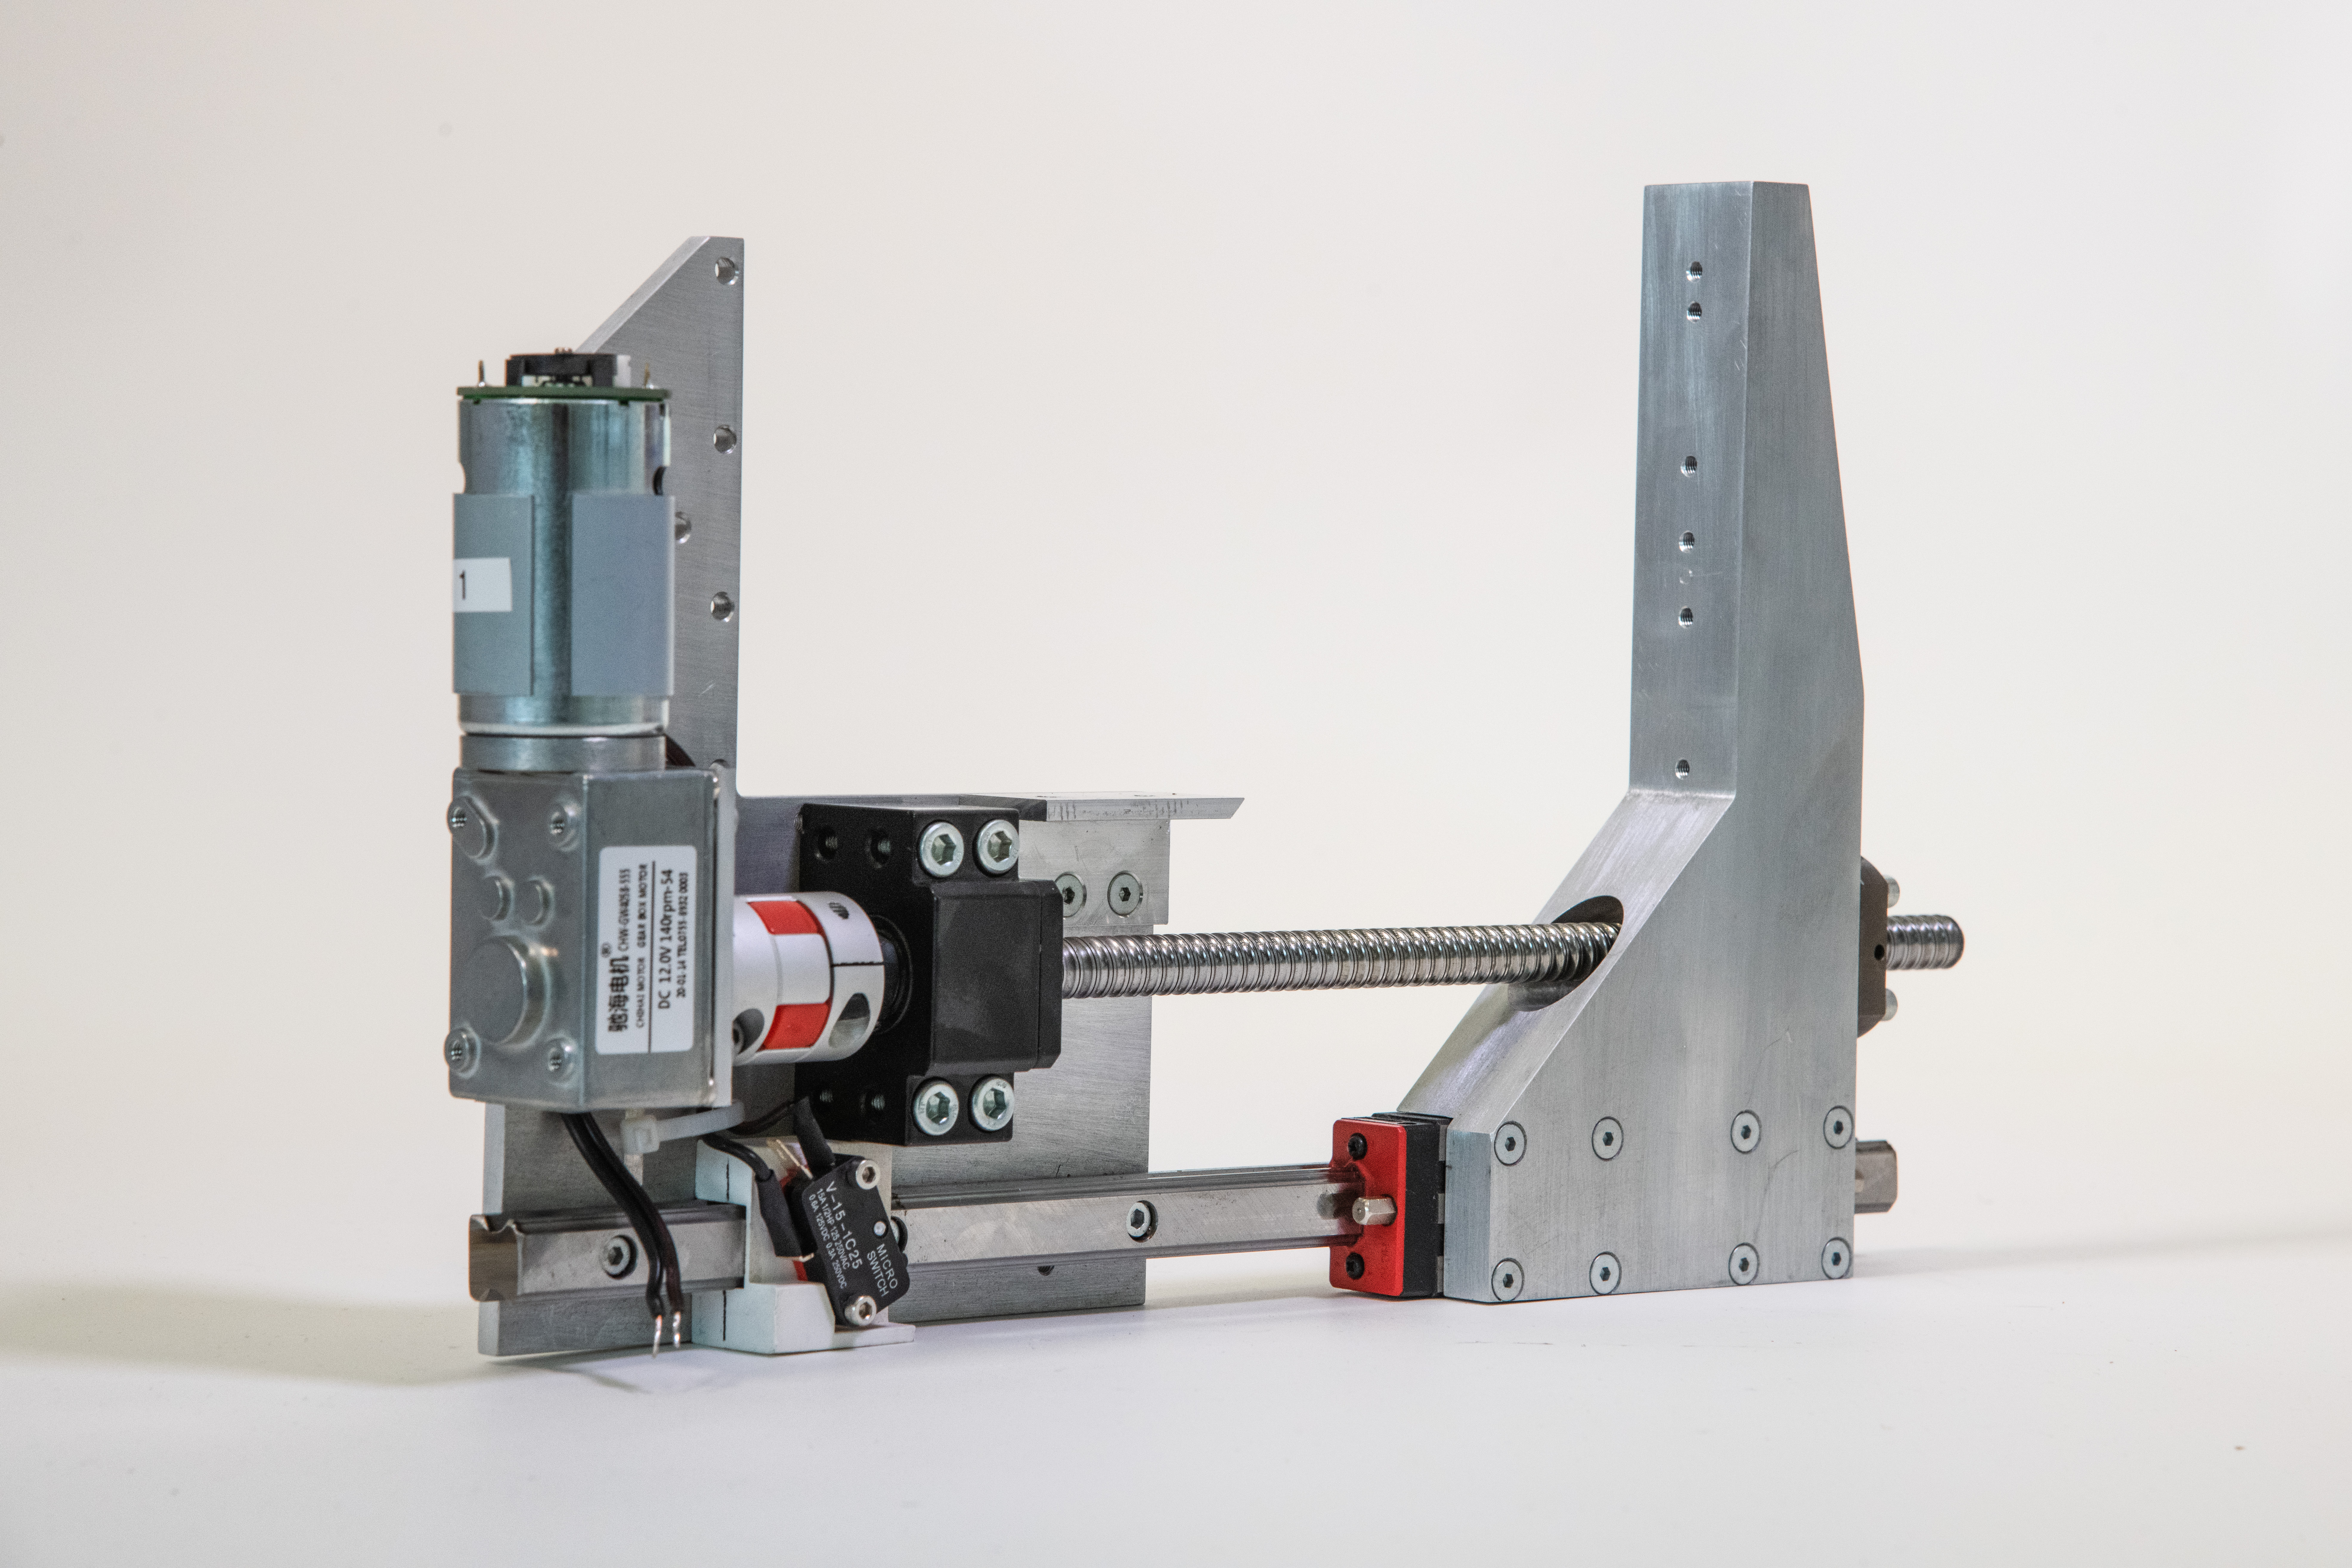
\includegraphics[width=0.99\textwidth]{images/05/image35.jpg}
    \caption{Actuator and jaw assembled for CL2 but later adapted to CL3}
    \label{fig:cl2-construction-photo}
\end{figure}

\subsection{Lap Clamp CL3 Hardware}
\label{subsection:exploration-2-lap-clamp-cl3-hardware}

The Lap Clamp CL3 was designed almost at the same time as CL2. The main intention is to adapt the clamping mechanism for variable-angle lap joints that was found to be of high importance in previous explorartion round \seeref{subsection:exploration-2-parametric-variations-of-lap-joints}. 

The initial goal is to create a clamp that can accommodate 45 degrees lap joints that are commonly used in diagonal bracing. However, in the process of adapting the clamp, it is found that the best strategy is to separate the hardware for left-handed joint and right-handed joint angles. This resulted in two clamp designs that are mirror-symmetrical, each able to handle 25 to 90 degrees on each side (measured on the acute angle of the intersection). 

\paragraph{Design Considerations}

Figure \ref{fig:cl3-design-steps} illustrates the evolution from the two-jaw CL2 design (\ref{fig:cl3-design-step-1}) towards a single-jaw design (\ref{fig:cl3-design-step-4}) that can be used for an angled lap joint. The main difference is the change of pressure location from the side of the joint towards the centre of the joint, where the two beams intersect.

\begin{figure}
    \centering
    \begin{subfigure}[b]{0.49\textwidth}
        \centering
        \includegraphics[width=\textwidth]{images/05/cl2-iteration-1.jpg}
        \caption{Design iteration 1}
        \label{fig:cl3-design-step-1}
    \end{subfigure}
    \hfill
    \begin{subfigure}[b]{0.49\textwidth}
        \centering
        \includegraphics[width=\textwidth]{images/05/cl2-iteration-2.jpg}
        \caption{Design iteration 2}
        \label{fig:cl3-design-step-2}
    \end{subfigure}
    \vskip\baselineskip % Next row
    \begin{subfigure}[b]{0.49\textwidth}
        \centering
        \includegraphics[width=\textwidth]{images/05/cl2-iteration-3.jpg}
        \caption{Design iteration 3}
        \label{fig:cl3-design-step-3}
    \end{subfigure}
    \hfill
    \begin{subfigure}[b]{0.49\textwidth}
        \centering
        \includegraphics[width=\textwidth]{images/05/cl2-iteration-4.jpg}
        \caption{Design iteration 4}
        \label{fig:cl3-design-step-4}
    \end{subfigure}
    \caption[Design iteration of the CL3 Clamp]
    {Design iteration of the CL3 Clamp showing different jaw positioning strategies}
    \label{fig:cl3-design-steps}
\end{figure}

Figure \ref{fig:cl3-docking-adapter-design} shows the location of the clamp attachment gripper and the docking adapter being changed from the back of the joint (\ref{fig:l3-docking-adapter-1}) to the side of the joint in the obtuse angle quadrant (\ref{fig:l3-docking-adapter-2}). Because the new attachment gripper closes in the front-back direction instead of the left-right direction, the choice of the actuator was also changed from a self-centering pneumatic gripper to a pneumatic linear slide.

% 2 Horizontal Image  
\begin{figure}
    \centering
    \begin{subfigure}[b]{0.49\textwidth}
        \centering
        \includegraphics[width=\textwidth]{images/05/cl3-docking-old.jpg}
        \caption{Docking adapter at the back}
        \label{fig:l3-docking-adapter-1}
    \end{subfigure}
    \hfill
    \begin{subfigure}[b]{0.49\textwidth}
        \centering
        \includegraphics[width=\textwidth]{images/05/cl3-docking.jpg}
        \caption{Docking adapter at the side}
        \label{fig:l3-docking-adapter-2}
    \end{subfigure}
    \caption{Design iteration of the docking adapter and hanging gripper of the CL3 clamp}
    \label{fig:cl3-docking-adapter-design}
\end{figure}

Figure \ref{fig:cl3-cl3m-mirror-design} shows the design of the two mirror-symmetrical clamps, named CL3 and CL3M. The symmetrical clamp jaws are adapted from the left and right jaw of the CL2 construction. The position of the docking adapter provided ample room for the robotic arm to attach it to the structure (Figure \ref{fig:cl3-robot-detach-1}) and detach it after use (Figure \ref{fig:cl3-robot-detach-2}). 

\begin{figure}
    \centering
    \includegraphics[width=0.99\textwidth]{images/05/cl3-mirror-design.jpg}
    \caption[Mirror design of the CL3 and CL3M clamp]{Mirror design of the CL3 (left) and CL3M (right) clamp}
    \label{fig:cl3-cl3m-mirror-design}
\end{figure}

% 2 Horizontal Image  
\begin{figure}
    \centering
    \begin{subfigure}[b]{0.49\textwidth}
        \centering
        \includegraphics[width=\textwidth]{images/05/image51.jpg}
        \caption{Robotic arm placing clamp on joint}
        \label{fig:cl3-robot-detach-1}
    \end{subfigure}
    \hfill
    \begin{subfigure}[b]{0.49\textwidth}
        \centering
        \includegraphics[width=\textwidth]{images/05/image21.jpg}
        \caption{Clamp detached from timber joint}
        \label{fig:cl3-robot-detach-2}
    \end{subfigure}
    \caption{Diagram showing the attach and detach operation of CL1 Clamp with robotic arm}
    \label{fig:cl3-robot-detach}
\end{figure}


\paragraph{Design Details}

Figure \ref{fig:diagram-cl3-front} and \ref{fig:diagram-cl3-back} shows the main components of the final CL3 clamp design after auxiliary components are added. The components on the CL3M are similar.

\todo{Labels added to figure of CL3}

\begin{figure}
    \centering
    \includegraphics[width=0.99\textwidth]{images/05/cl3-design-front-label.jpg }
    \caption{Front side of CL3 clamp design with component labels}
    \label{fig:diagram-cl3-front}

    \centering
    \includegraphics[width=0.99\textwidth]{images/05/cl3-design-back-labels.jpg
    }
    \caption{Back side of CL3 clamp design with component labels}
    \label{fig:diagram-cl3-back}
\end{figure}

\paragraph{Construction}

Because of the vastly superior support for variable-angle lap joints, the CL3 was constructed in favour of the CL2 design. This was a risky decision because the single-jaw and slider-based gripper strategy was a large jump from the CL1 prototype. Nevertheless, two copies of the CL3 and CL3M designs were constructed. The decision to make four clamps was a balance between cost and sufficient design freedom for creating the demonstrator.

Figure \ref{fig:photo-cl3-front} and \ref{fig:photo-cl3-back} below shows the constructed CL3 clamp before the docking adapter was attached. This was because the demonstration goal in this round did not include the robotic attachment and detachment yet. A manual pneumatic connector can be seen attached for the operator to operate the gripper manually.

\begin{figure}
    \centering
    \includegraphics[width=0.99\textwidth]{images/05/CL3_Back.jpg}
    \caption{Front side photo of CL3 Clamp}
    \label{fig:photo-cl3-front}

    \centering
    \includegraphics[width=0.99\textwidth]{images/05/CL3_Front.jpg}
    \caption{Back side photo of CL3 Clamp}
    \label{fig:photo-cl3-back}
\end{figure}

\FloatBarrier

\subsection{Docking adapter}
\label{subsection:exploration-2-docking-adapter}

The docking adapter is the mechanical interface that serves as the connection between the robotic arm and the DiRT tools. In the initial concept, this is similar to a robotic quick changer that is commonly used in the manufacturing industry for switching between tools. Because there was a set of robotic quick changers (SWK / SWA 040 series by Schunk GmbH \& Co. KG, Global) available in the lab donated by previous projects, it was adopted for this role. Figure \ref{fig:quick-changer} shows the quick changer mounted on the flange of the robot. Two pneumatic feed through can be seen connected for the parallel grippers \seeref{subsection:exploration-2-parallel-gripper-pg500-and-pg1000} and to actuate the hanging gripper on the clamps.


\begin{figure}
    \centering
    \includegraphics[width=0.99\textwidth]{images/05/image20.jpg}
    \caption{Photo of robotic quick changer mounted on the robot flange}
    \label{fig:quick-changer}
\end{figure}

\todo{Below: paragraph revised to add a quick explanation about why the docking adapter is not ideal.}

The choice of this robotic quick changer was known to be a risky decision because the allowable payload of 50kg is close to the combined weight of a long beam and a large gripper. However it was only after using this robotic quick changer, that another property was found to be unideal for the docking adapter role. This is related to the maximum permissible offset of 2mm being too demanding for accurate alignment. For DiRT operations, especially for timber assembly, this accuracy is hard to achieve. Despite its limitations, this robotic quick changer is used until the end of this thesis. The related problems are documented \seerefii{subsection:exploration-3-docking-adapter-misalignment}{subsection:exploration-3-docking-adapter-fail-to-lock}. This eventually led to the development of multiple workarounds for improving alignment accuracy \seerefii{subsection:exploration-3-docking-adapter-alignment-with-camera}{subsection:exploration-4-camera-marker-alignment-correction-system} and the reliability of the lock actuation \seerefii{subsection:exploration-4-compliant-control-for-robotic-arm}{subsection:exploration-5-automatic-shake-when-docking-with-tools}.

\subsection{Parallel Gripper PG500 and PG1000}
\label{subsection:exploration-2-parallel-gripper-pg500-and-pg1000}

The Parallel Gripper PG500 and PG1000 were designed to allow the robotic arm to hold timber beams of different lengths. The design of these grippers was adopted from a previous project in the laboratory that was proven to be reliable. 

Figure \ref{fig:rendering-pg1000} shows the main components of the Parallel Gripper PG1000. It consists of two self-centring parallel pneumatic grippers positioned 950mm apart (measured on the centre). An aluminium bar provides the support of the two grippers with the docking adapter mounted on top. The total length of the gripper is 1005mm. Figure \ref{fig:rendering-pg1000-dimension} below shows the dimensions of the gripper (including both sides of the robotic quick changer) in its closed state. The design of the PG500 is similar but with a shorter connecting bar. 

\begin{figure}
    \centering
    \includegraphics[width=0.99\textwidth]{images/05/image7.jpg}
    \caption{Rendering of PG1000 Parallel Gripper}
    \label{fig:rendering-pg1000}
\end{figure}


\begin{figure}
    \centering
    \includegraphics[width=0.90\textwidth]{images/05/image87.jpg}
    \caption{Major dimension of PG1000 Parallel Gripper}
    \label{fig:rendering-pg1000-dimension}
\end{figure}

These timber beams used for the demonstration have a fixed 100mm square profile. This allows the use of the short-stroke pneumatic gripper (PGN-plus 100-1 by Schunk) that has a compact design. The stroke is 10mm on each jaw with a combined closing force of 900N. 

\paragraph{Construction}

Figure \ref{fig:photo-pg500} shows the constructed PG500 Parallel Gripper. Sandpaper can be seen lining the gripper fingers to prevent the wood from slipping. The GP1000 has a similar construction. 

\begin{figure}
    \centering
    \includegraphics[width=0.99\textwidth]{images/05/image42.jpg}
    \caption{Photo of PG500 Parallel Gripper}
    \label{fig:photo-pg500}
\end{figure}

\subsection{CL3 Clamp Drive Electronics}
\label{subsection:exploration-2-cl3-clamp-electronics}

The CL3 Clamp Drive Electronics was based on the experience learnt from the CL1 electronics. The new design features the following improvements:

\begin{itemize}[nosep]
    \item \textbf{Arduino Nano} was used instead of Arduino Uno. It offers the same capabilities in a more compact form factor.
    \item \textbf{A buffer diode} is added before battery voltage regulation to address the brownout problem \seeref{subsection:exploration-1-electronics-brownout}.
    \item \textbf{Pin assignment} supports controlling 1 or 2 DC Servo motors. 
    \begin{itemize}
        \item The one-motor scenario is designed for CL3 hardware with one clamp jaw. \seeref{subsection:exploration-2-lap-clamp-cl3-hardware}
        \item The two-motor scenario is reserved for CL2 hardware but was never needed or tested because CL3 was successful.
    \end{itemize}
    \item \textbf{Connection between the controller and motor driver} was changed to a ribbon cable to be more flexible with positioning.
\end{itemize}

The CL3 clamp drive electronics were designed with the following new features:

\begin{itemize}[nosep]
    \item \textbf{Wireless Control and Communication} through CC1101 radio module over SPI bus. \seeref{subsection:exploration-2-radio-network}
    \item \textbf{Device MAC address} can be set by a physical DIP Switch
    \item \textbf{End / Homing Switch} input monitoring 
    \item \textbf{Integrated Plastic Enclosure} 3D printed with PLA plastic
\end{itemize}

\paragraph{Design Considerations}

The main challenge in developing this electronic controller is the limited amount of IO pins available from the Arduino Nano. Due to the addition of the radio module and two limit switches, almost all IO pins are occupied. Even the design of the DIP switch input to set the Radio MAC address had to be compressed to occupy only a single analogue input pin by using a resistor ladder. \parencite{chrisPerfectMultibuttonInput2018}

The load cell connection that was included in the CL1 design was removed because of the lack of pins. This is a difficult compromise because the load cell could have provided useful insight for better understanding the synchronised clamping process. As there was no chance to test the load cells in the previous round, they were considered a lower priority than switching to a different microcontroller with more GPIO pins.
Table \ref{table:cl3-clamp-electronics-components} shows the main components. The underlined items are newly added in this exploration round. 

\begin{table}
    \includegraphics[page=6, trim=25.4mm 185mm 25.4mm 33mm, clip, width=0.98\textwidth]{tables/Tables in Chapter 5.pdf}
    \caption{New components in the CL3 Clamp Drive Electronics}
    \label{table:cl3-clamp-electronics-components}
\end{table}

\textbf{The end switch} was newly added because the previous linear actuator had integrated end switches that would simply disconnect the DC motor when reaching the end. This arrangement introduced unnecessary uncertainty to the control firmware because it is not possible to determine whether the motor had stalled due to load or whether it reached the end of travel.

\textbf{The DIP switch} was added to enable the physical setting of the MAC address for each of the four controllers. This simplified the firmware uploading process because the MAC addresses do not have to be changed for individual compilation. An alternative solution could have involved storing the MAC address in the microcontroller's EEPROM. In practice, the DIP Switch was set only once and was never adjusted. 

\textbf{The plastic enclosure} was designed specifically for the CL3 clamp body. It consists of two parts - a base for the circuit boards to attach to the metallic body of the clamp and a cover that can be easily removed for maintenance without detaching the base. The design of stacking the main circuit board above the motor driver board was kept from the CL1 design in order to keep the device compact. 

In cases where the entire electronic pack had to be removed from the clamp, it can be easily separated without affecting the mechanical parts. The plastic enclosures are slightly different due to the symmetrical difference between CL3 and CL3M clamps. 

\textbf{Plug connectors} were used for the motor and encoder. Connection terminals were used for the end switches. This proved to be beneficial on multiple occasions where it was necessary to separate the motors and end switches for maintenance or repair.

\paragraph{Schematics and Construction}

\begin{figure}
    \centering
    \includegraphics[width=0.99\textwidth]{images/05/image61.jpg}
    \caption{Schematics of the CL3 clamp drive electronics}
    \label{fig:schematic-cl3-clamp-electronics}
\end{figure}


The schematics of the CL3 clamp drive electronics is shown in Figure \ref{fig:schematic-cl3-clamp-electronics}.
Four identical controller boards were made for the CL3 and CL3M clamps. The circuit is built on a 60mm x 80mm protoboard and manually wired by the author similar to the previous CL1 board. Figure \ref{fig:board-cl3-clamp-electronics} shows the wiring underneath the protoboard and the jumpers that route directly between pins.

% 2 Horizontal Image  
\begin{figure}
    \centering
    \begin{minipage}{0.55\textwidth}
        \centering
        \includegraphics[width=\textwidth]{images/05/image79.jpg}
        \caption{Design drawing of the CL3 circuit board with jumpers and wiring}
        \label{fig:board-cl3-clamp-electronics}
    \end{minipage}
    \hfill
    \begin{minipage}{0.43\textwidth}
        \centering
        \includegraphics[width=\textwidth]{images/05/image18.jpg}
        \caption{Integrated plastic enclosure for the CL3 clamp drive electronics}
        \label{fig:plastic-enclosure-cl3-clamp-electronics}
    \end{minipage}
\end{figure}

Despite the relatively low complexity, a lesson learnt from this experience is that the time spent to wire and debug a protoboard is better worth outsourcing the build to a PCB foundry. 

\textbf{The plastic enclosure is 3D-printed} with PLA plastic using a generic desktop 3D printer with 0.2mm layer height and 90\% infill. The design of the plastic enclosure is shown in Figure \ref{fig:plastic-enclosure-cl3-clamp-electronics}. 

Figure \ref{fig:photo-cl3-clamp-electronics} shows the main components on the circuit board.
Figure \ref{fig:photo-cl3-with-electronics-installed} shows the electronics enclosure as it is installed on the CL3 hardware. It was printed in black PLA and has a slightly different design to fit the clamp better.
In the subsequent robotic demonstrations, the protection proved to be invaluable for avoiding collision damage to fragile components.

\begin{figure}
    \centering
    \includegraphics[width=0.99\textwidth]{images/05/image31.jpg}
    \caption{Photo of the CL3 clamp drive electronics with plastic enclosure}
    \label{fig:photo-cl3-clamp-electronics}
\end{figure}

\begin{figure}
    \centering
    \includegraphics[width=0.99\textwidth]{images/05/image64.jpg}
    \caption{Photo of the electronic module installed on the back of the CL3 clamp}
    \label{fig:photo-cl3-with-electronics-installed}
\end{figure}

\FloatBarrier

\subsection{Motion Control for DC Servo Motor}
\label{subsection:exploration-2-motion-control-for-dc-servo-motor}

The motion control algorithm for the DC motor is an important development for creating the CL3 Clamp firmware (an L1 controller). It is a trjectory controller that implements a trapezoidal motion profile \seeref{subsection:exploration-2-synchronisation-between-clamp-and-rfl-robot}. The algorithm consists of three parts as shown in Table
\ref{table:motion-control-algorithm}.

\begin{table}[h]
    \includegraphics[page=7, trim=25.4mm 195mm 25.4mm 33mm, clip, width=0.98\textwidth]{tables/Tables in Chapter 5.pdf}
    \caption{New components in the CL3 Clamp Drive Electronics}
    \label{table:motion-control-algorithm}
\end{table}

\FloatBarrier

The development process required multiple experiments to validate the system and determine suitable operation parameters. The following list shows the experiments and their results in chronological order.

\begin{enumerate}[nosep]
\item Validation of the encoder
    \begin{itemize}
        \item Confirmed the accuracy of the microcontroller integrating encoder signals in both directions
    \end{itemize}
    \item DC voltage and motor speed relationship
    \begin{itemize}
        \item Confirmed the motor driver can deliver power within limits
    \end{itemize}
    \item PWM control (open loop)
    \begin{itemize}
        \item Established suitable PWM Frequency for a linear duty cycle to motor speed relationship
        \item Established the PWM deadband in speed control
    \end{itemize}
    \item PID Speed Control (closed loop with encoder)
    \begin{itemize}
        \item Validated deadband linearity over zero crossing for bidirectional control
    \end{itemize}
    \item Rectangular motion profile (closed-loop with respect to a step function)
    \begin{itemize}
        \item Established PID values for improving motor control damping
    \end{itemize}
    \item Trapezoidal motion profile
    \begin{itemize}
        \item Established acceleration, deceleration, and maximum speed values for operations
        \item Established the maximum tracking error useful for determining a stalled condition
    \end{itemize}
    \item Stopping condition (indirectly provides stall protection to the motor)
    \begin{itemize}
        \item Validated position error monitoring strategy
        \item Validated pull force is unaffected by stopping condition
    \end{itemize}
\end{enumerate}

\FloatBarrier

\paragraph{Operational Parameters}

Table \ref{table:motion-control-parameters-cl3} lists the operation parameters that were obtained from the tests and used in the CL3 Firmware.

\begin{table}[h]
    \includegraphics[page=8, trim=25.4mm 135mm 25.4mm 33mm, clip, width=0.98\textwidth]{tables/Tables in Chapter 5.pdf}
    \caption{Motion control parameters for the CL3 clamp}
    \label{table:motion-control-parameters-cl3}
\end{table}

\FloatBarrier

\paragraph{Validation}

Figure \ref{fig:cl3-validation-motion-profile} shows the tracking performance of the tuned controller. The blue line in the two graphs below shows the position and tracking error using the operation parameters listed above. The tracking error is within 10 encoder steps during the whole motion profile. This corresponds to 0.017mm for the ballscrew with 4mm lead, which is a negligible error.

Figure \ref{fig:cl3-validation-clamping-force} shows the clamping force of the clamp jaw. The solid purple line in the graph below shows the pull force under different maximum speed settings. The results between 1000 and 3000 step/s are similar. This corresponds to the anticipated operation speed between 1.7mm/s and 5mm/s for the ballscrew with 4mm lead.

% 2 Horizontal Image  
\begin{figure}[!htp]
    \centering
    \begin{subfigure}[b]{0.49\textwidth}
        \centering
        \includegraphics[width=\textwidth]{images/05/image85.jpg}
        \caption{Position over Time}
        \label{fig:cl3-validation-position}
    \end{subfigure}
    \hfill
    \begin{subfigure}[b]{0.49\textwidth}
        \centering
        \includegraphics[width=\textwidth]{images/05/image22.jpg}
        \caption{Tracking Error over Time}
        \label{fig:cl3-validation-error}
    \end{subfigure}
    \caption{Validated tracking performance of the CL3 controller}
    \label{fig:cl3-validation-motion-profile}
\end{figure}

\begin{figure}[!htp]
    \centering
    \includegraphics[width=0.90\textwidth]{images/05/image52.jpg}
    \caption{Validated clamping force of the CL3 clamp}
    \label{fig:cl3-validation-clamping-force}
\end{figure}

\FloatBarrier

\subsection{CL3 Firmware}
\label{subsection:exploration-2-cl3-firmware}

The CL3 Firmware is an L1 controller developed to run on the Arduino microcontroller. It serves two primary purposes.

\begin{itemize}[nosep]
    \item Receive and process commands (Serial and Radio)
    \item Controlled servo motor motion
\end{itemize}

The main loop implemented quasi-time-sharing task management to service different subroutines. This requires all the subroutines to execute in a relatively short amount of time. All blocking functions, such as waiting for a serial message to arrive to transmit, have to be implemented in an asynchronous way. The table below contains all the subroutines, they are all visited in each control loop.

\begin{table}[h]
    \includegraphics[page=9, trim=25.4mm 200mm 25.4mm 33mm, clip, width=0.98\textwidth]{tables/Tables in Chapter 5.pdf}
    \caption{Subroutines in the CL3 Firmware}
    \label{table:cl3-firmware-subroutines}
\end{table}

\subsection{Radio Network}
\label{subsection:exploration-2-radio-network}

The DiRT radio network is developed to create a reliable communication network with the following properties:

\begin{itemize}[nosep]
    \item Low latency
    \item Insensitive to electromagnetic noise emitting from the robotics environment
    \item Insensitive to occlusion from the construction environment
\end{itemize}

The initial attempt of using a 2.4Ghz WiFi network from an Arduino microcontroller yielded poor results. The main problem is the reconnection time after a dropped connection is too long for the robotic operation, and its high frequency is fairly sensitive to occlusion by metallic objects. ZigBee technologies were considered for creating this network because of their integrated solution for the physical radio and network layer. However, I decided to implement the network for the opportunity to understand the underlying mechanism better and to have more control over the parameters of the radio and the network.

\begin{figure}
    \centering
    \includegraphics[width=0.99\textwidth]{images/05/image56.jpg}
    \caption{Photo of the Telesky CC1101 radio module}
    \label{fig:photo-cc1101}
\end{figure}

My custom implementation consists of a single-chip digital packet radio, CC1101 by Texas Instrument, that is capable of managing the physical layer \parencite{texasinstrumentsCC1101LowPowerSub12023}. The surface mount ship can be interfaced easily through an integrated module manufactured by Telesky (Figure \ref{fig:photo-cc1101}). The network is implemented with a star topology with a PC acting as the network coordinator. This PC connects to the network through an Arduino-based network adapter \seeref{subsection:exploration-2-radio-network-usb-dongle-adapter}. All the clamps are connected to the network by a direct connection between the CC1101 chip and the Arduino microcontroller. 

Communication over the network is always initiated by the controlling PC, even for telemetry updates. Every clamp has a fixed MAC (Media Access Control) address that is registered to the L2 Clamp Controller \seeref{subsection:exploration-2-clamp-controller-l2} on the PC and their identity is known by it. Therefore, there is no need for any network discovery or handshake for the clamps to join the network. During the robotic assembly operation, all clamps are expected to be present in the network, and their response to a telemetry request is sufficient to prove their existence on the network. This design eliminated the overhead and delay for a clamp to rejoin the network.

The transport layer design is also customised to the unique operation of the devices. In order to reduce latency and maximise throughput, all the commands and response over the network is designed to fit within one single flexible-length data packet that is between 10 to 30 bytes long. This avoided the delay when reassembling messages. 


\begin{table}
    \includegraphics[page=10, trim=25.4mm 65mm 25.4mm 33mm, clip, width=0.98\textwidth]{tables/Tables in Chapter 5.pdf}
    \caption{Physical and Network Layer Techniques for the Radio Network}
    \label{table:radio-network-physical-and-network-layer-techniques}
\end{table}

Automatic resend was implemented in the application layer in the L2 controller but not on the clamp firmware. In the case where a clamp does not acknowledge a command, the PC can resend it after a fixed amount of time. 

Other physical and network layer techniques that were considered for improving the reliability and performance of the network are listed in Table \ref{table:radio-network-physical-and-network-layer-techniques}, including the reasons whether they were adopted or not.

The development of the network is tested with a throughput tester inside the RFL robotic environment separate from the development of the clamp drive electronics and firmware. The testing setup consists of a base station PC with the radio adapter over USB, and a battery powered Arduino connected to the radio module providing a response. This setup simulates a complete round trip for the command and response application. A number of the testing scenarios were performed to tune operation parameters and validate the reliability of the system. Below is a summary of the results:

\begin{itemize}
    \item \textbf{Packet length vs round trip time}
    \begin{itemize}
        \item Different packet lengths from 1 byte to 59 bytes were tested 100 times, no-acknowledge is not counted. Figure \ref{fig:roundtrip-time} shows the measured round trip time. It appears to be highly linear in relation to the packet length (linear fit: y = 0.3906x + 12.108). Every byte corresponds to roughly 0.39ms to do one round trip, which is equatable to the default 38kbps modem setting on the chip. The 12.1ms offset includes the overhead of the Arduino microcontroller and the USB serial port.
        \item This test confirms that there are no buffering issues within the round trip and the frequency channel is mostly clear for immediate transmission.
        \item In our application, packet length will not exceed 59 bytes. Therefore a 40ms wait duration is set for a message without acknowledgement to be considered a lost packet.
    \end{itemize}
    \item \textbf{Obstacle penetration}
    \begin{itemize}
        \item Test successfully performed over 5m distance with 2 closed doors in between. Using a packet length of 20 bytes, the result is less than 1\% packet loss.
    \end{itemize}
    \item \textbf{433 MHz vs 868MHz}
    \begin{itemize}
        \item Tests have shown that the 433MHz outperforms the 868 MHz significantly in range and occlusion tests. However, it is hard to draw a conclusion whether this is due to the lower frequency or because the integrated radio module is designed with peripheral components optimised for 433MHz operations.
    \end{itemize}
\end{itemize}

\begin{figure}[h]
    \centering
    \includegraphics[width=0.99\textwidth]{images/05/image108.png}
    \caption{Packet length vs round trip time}
    \label{fig:roundtrip-time}
\end{figure}

The development of this radio network ended after these validation tests and it was used without issues for all subsequent demonstrations. However, later observations \seeref{subsection:exploration-5-wireless-radio-latency} indicates that the latency of the wireless communication system may pose a limit to a larger DiRT system.

\subsection{Radio Network USB Dongle Adapter}
\label{subsection:exploration-2-radio-network-usb-dongle-adapter}

The USB Dongle adapter is the physical network layer that allows the L2 clamp controller running on a personal computer (PC) to send commands to the clamps. Most of the functionalities are implemented on its firmware running on the microcontroller:

\begin{itemize}[nosep]
    \item Allow the PC to connect to it via USB port.
    \item Allow the PC to configure the CC1101 settings via the USB (address, frequency, channel and sync word)
    \item Allow the PC to send and receive variable-length message packet via the USB
    \item Allow debug messages to be printed to a 1602 LCD Screen (via I2C bus with the PCF9574 IO Expander)
    \begin{itemize}
        \item Used only in debug and development scenarios as its use reduces the adapter throughput.
    \end{itemize}
\end{itemize}

\paragraph{Design and Construction} \ref{fig:schematic-radio-network-usb-dongle-adapter}.
The USB Dongle Adapter is based on the Arduino Nano microcontroller. It is a compact design that is capable of providing all the functionalities required for the adapter. The main components are listed in Table \ref{table:radio-network-usb-dongle-adapter-components}. The schematic design is very simple as shown in Figure \ref{fig:schematic-radio-network-usb-dongle-adapter}.


\begin{figure}[h]
    \centering
    \includegraphics[width=0.99\textwidth]{images/05/image72.jpg}
    \caption{Schematics of the radio network USB dongle adapter}
    \label{fig:schematic-radio-network-usb-dongle-adapter}
\end{figure}


\begin{table}
    \includegraphics[page=11, trim=25.4mm 185mm 25.4mm 33mm, clip, width=0.98\textwidth]{tables/Tables in Chapter 5.pdf}
    \caption{Main components of the radio network USB dongle adapter}
    \label{table:radio-network-usb-dongle-adapter-components}
\end{table}


The circuit is built on a 50mm x 70mm protoboard housed inside an unremarkable 3D-printed plastic enclosure. The wiring is completed using small wires. Arrangement of the components can be seen in Figure \ref{fig:photo-radio-network-usb-dongle-adapter}. Two copies of the design was constructed (one acting as a spare) and validated similar to the round-trip-test that was performed for the radio network. \seeref{subsection:exploration-2-radio-network}

\begin{figure}[h]
    \centering
    \includegraphics[width=0.99\textwidth]{images/05/image12.jpg}
    \caption{Photo of the radio network USB dongle adapter}
    \label{fig:photo-radio-network-usb-dongle-adapter}
\end{figure}

\FloatBarrier

\subsection{Clamp Controller (L2)}
\label{subsection:exploration-2-clamp-controller-l2}

The Clamp controller is a L2 controller that is developed to run on the controlling PC for supervising all the clamps. It provides the following functions:

\begin{itemize}[nosep]
    \item \textbf{Provides a GUI overview} of all Clamps and their telemetry
    \item \textbf{ROS messaging} Accepts commands from Level 3 Process Controller over ROS messaging network using \verb|ros_bridge| as interface.
    \begin{itemize}
        \item Go to Position Command (Format: \verb|[clamp_ids],velocity,position_mm|)
        \item Stop Command (Format: \verb|[clamp_ids]|)
    \end{itemize}
    \item \textbf{Connects to the Clamp Radio Network} using the USB Radio Dongle via Serial Port. Sends commands to each individual clamp:
    \begin{itemize}
        \item Set Velocity Command (Format: \verb|clamp_id,velocity_step_per_sec)|
        \item Go to Position Command (Format: \verb|clamp_id,position_step|)
        \item Stop Command (Format: \verb|clamp_id|)
    \end{itemize}
    \item \textbf{UI buttons for manual operations} to either one or all clamps:
    \begin{itemize}
        \item Homing (on start of the device)
        \item Go to a position
        \item Set Active Velocity
        \item Stop
    \end{itemize}
    \item Log traffic
\end{itemize}

Figure \ref{fig:screenshot-clamp-controller-gui} shows the GUI when it is configured for 2 clamps during testing. 

\begin{figure}
    \centering
    \includegraphics[width=0.99\textwidth]{images/05/image39.jpg}
    \caption{Screenshot of the Clamp Controller GUI}
    \label{fig:screenshot-clamp-controller-gui}
\end{figure}

\paragraph{Telemetry}

In order to avoid radio contention, a telemetry update is actively requested by the L2 Controller. The request interval is 150ms for clamps that are in active motion. Otherwise, the update is every 2000ms. 

In order to reduce processing time in the L1 controller, telemetry is transmitted from the L1 Firmware to L2 Clamp Controller in raw values. A digital twin model was used to keep track of the conversion scale between the raw values and their output.

\begin{itemize}[nosep]
    \item Current Velocity, Current Position, Target Position, Error
    \item Motor Power Output
    \item Battery Value 
\end{itemize}

\paragraph{Automatic Resend Request (ARQ)}

In this exploration round, all the commands between L3, L2 and L1 controllers are implemented as single-direction communication. There are no mechanisms designed to provide feedback on the execution status such as \textit{running} or \textit{completed} or \textit{failed}. However, communication between L2 and L1 controllers is wireless, and it has a high chance of lost packages. Therefore an acknowledgement and automatic repeat request (ARQ) protocol were implemented in the L2 and L1 controllers. The recent protocol has two parameters, \textit{acknowledgement} time before resending and the \textit{number of attempts}. The default values used for motion commands are 100ms and 4 attempts. The values used for requesting telemetry are 40ms and 1 attempt. 

\subsection{Assembly Model Data Structure and Functions}
\label{subsection:exploration-2-assembly-model-data-structure-and-functions}

In order to support the robotic assembly process, a data structure was developed to support CAD modelling of the beams, joints and their assembly. It was designed to facilitate various geometrical operations, such as inferring joints from beam arrangements, and topographical operations among beams and neighbours \seeref{subsection:exploration-2-cad-modelling}. The data structure is based on the object-oriented programming paradigm and implemented in Python. The three main entities in the data structure are Beam, Joint and Assembly:

\begin{description}
    \item [Beam] Represents the physical beam, with a one-to-one correspondence.
    \item [Joint] Represents two properties 
    \begin{itemize}
        \item the physical joints that are carved into the beam
        \item the topological connection between beams in the structure
    \end{itemize}
    \item [Assembly] Represents a group of beams (typically that are connected by joints)
\end{description}

\subsubsection{Beam and Joint}
\label{subsubsection:exploration-2-beam-and-joint}

While Beam objects have a one-to-one relationship to a physical entity, the Joint object serves a dual purpose of representing geometry and relationships. Figure \ref{fig:diagram-two-possible-data-structures} shows two possible structures to represent Joints as a graph. The difference between representation (a) and (b) is whether the Joint is represented as one or two objects in between two beams.

\begin{figure}[!h]
    \centering
    \includegraphics[width=0.99\textwidth]{images/05/image59.pdf}
    \caption{Diagram showing two possible data structures to represent Joints as a graph}
    \label{fig:diagram-two-possible-data-structures}
\end{figure}



After considering the compatibility with BTLx, a leading file format for exchanging geometry data for timber components, representation (a) was chosen. This is because the double-joint structure is similar to the Beam-to-Processing relationship used in BTLx, which also facilitates the separation of the geometrical entities for each individual beam. Figure \ref{fig:diagram-graph-can-be-sliced} shows how the graph in representation (a) can be sliced to create a geometry group for each beam.


\begin{figure}[!h]
    \centering
    \includegraphics[width=0.99\textwidth]{images/05/image73.pdf}
    \caption{Diagram showing how the graph can be sliced into individual beams}
    \label{fig:diagram-graph-can-be-sliced}
\end{figure}


The geometry of the beam with joints can be computed by solid boolean operations between the un-cut beam model, and the negative models of the joint volumes. The relative ease of dynamically recomputing the solid model allows quick visualisation during interactive design.

\begin{equation}
    \textrm{Geometry of Beam}[i] = \textrm{Uncut Model of Beam}[i] \setminus \bigcup_{j=1}^n  \textrm{Negative Volume Model of Joint}[j]
\end{equation}

Where: 
\begin{align*}
    i \quad &\textrm{is \quad the index of the beam}\\
    j \quad &\textrm{is \quad the index of the joints on the beam}[i]\\
    n \quad &\textrm{is \quad the total number of joints on the beam}[i]\\
    \setminus \quad &\textrm{is \quad 3D Solid Boolean Subtraction Function}\\
    \bigcup \quad &\textrm{is \quad 3D Solid Boolean Union Function}
\end{align*}

This computation is also similar to the Beam and Processing relationships used in BTLx. The difference is that BTLx encodes a joint with a closer relationship to machine operations, such as removing the material with a mill head versus a saw.

\subsubsection{Assembly as a Graph}
\label{subsubsection:exploration-2-assembly-as-a-graph}

The Assembly object is a collection of Beams and Joints, and can be implemented as a graph structure. For example, (Figure \ref{fig:eextraction-of-beam-geometry}, left) shows the assembly graph using the two-joint-object arrangement. Two edges are used to connect between nodes, each of which can contain one of the joint objects. The extraction of the joint geometries related to a beam would be to select all the outward-going edges from it (Figure \ref{fig:eextraction-of-beam-geometry}, right).

\begin{figure}[!h]
    \centering
    \includegraphics[width=0.99\textwidth]{images/05/image68.pdf}
    \caption{Extraction of a beam's joint geometries from the assembly graph}
    \label{fig:eextraction-of-beam-geometry}
\end{figure}

\FloatBarrier

\paragraph{Assembly Sequence in Graph}

In order to support the modelling of the robotic assembly process, the graph used in this thesis is extended with a node property (a.k.a. beam property) for specifying its \textit{assembly sequence}. The property is a zero-index integer, and its values should be unique within an Assembly. Figure \ref{fig:assemble-sequence-added-to-the-assembly-graph} shows a structure below with four beams (A, B, C, D). The numbers in the bracket represent their assembly sequence. The Beam-Joint graph can be seen on the right.

\begin{figure}[!h]
    \centering
    \includegraphics[width=0.99\textwidth]{images/05/image103.pdf}
    \caption{Assembly sequence added to the assembly graph}
    \label{fig:assemble-sequence-added-to-the-assembly-graph}
\end{figure}

\FloatBarrier

\paragraph{Beam Deletion Operation}

Using the graph, it is possible to identify the neighbour relationships between beams. For example, if Beam B is to be removed, all the edges (joints) connecting to the B node should also be removed (see Figure \ref{fig:assembly-graph-deletion}). In addition, it is possible to identify the neighbours that are affected by the deletion (Beam C and D) and recompute downstream relationships only. 

\begin{figure}[!h]
    \centering
    \includegraphics[width=0.99\textwidth]{images/05/image103.pdf}
    \caption{Beam deletion operation on the assembly graph}
    \label{fig:assembly-graph-deletion}
\end{figure}

\FloatBarrier

\paragraph{Partially Assembled Structure}

Using this sequence number, it is possible to extract the partial structure at every step of the assembly. Figure \ref{fig:assembly-graph-slice-at-step} shows a visualization of the same structure in Figure \ref{fig:assemble-sequence-added-to-the-assembly-graph} but showing the state after three beams are installed. This graph slicing operation is common for visualisation \seeref{subsubsection:exploration-3-process-visualization-and-adjustment} and for using them as collision geometry during motion planning \seeref{subsubsection:exploration-3-compute-object-states}.

\begin{figure}[!h]
    \centering
    \includegraphics[width=0.99\textwidth]{images/05/image14.pdf}
    \caption{Slicing operation for visualzing a specific assembly step on the assembly graph}
    \label{fig:assembly-graph-slice-at-step}
\end{figure}

\FloatBarrier

\paragraph{Identify Mating Joints for Assembly}

For a given assembly step, It is also possible to identify the active beam and its joints that need to be assembled with the PA structure. For example, in the Figure \ref{fig:assembly-graph-identify-mating-joints}, Beam C(2) is the active beam for step 2. It has three outgoing edges in the graph (Joint C-A, C-B and C-D). Ignore the edges that are pointing to nodes (red) that have a higher sequence number (C-D). The remaining edges (green) are the joints that need to be assembled (Joint C-A and C-B). 

\begin{figure}[!h]
    \centering
    \includegraphics[width=0.99\textwidth]{images/05/image78.pdf}
    \caption{Identifying all mating joints for an assembly step on the assembly graph}
    \label{fig:assembly-graph-identify-mating-joints}
\end{figure}

\FloatBarrier

\paragraph{Assembly Sequence Modification}

It is also possible to perform more complex operations on the graph. For example, when swapping the order between two elements, identify the joints that need to be flipped. Figure \ref{fig:assembly-graph-change-sequence} shows an example where the sequence number of Beam C and D is swapped. Note that only the joints that are connecting the two swapped elements need to be flipped.

This swapping logic can be extended to pick a node and insert it at an arbitrary position in the assembly sequence.  The affected edges (joints) will be those whose nodes have flipped their earlier-later relationship. 

\begin{figure}[!h]
    \centering
    \includegraphics[width=0.99\textwidth]{images/05/image89.pdf}
    \caption{Operation to change assembly sequence in the assembly graph}
    \label{fig:assembly-graph-change-sequence}
\end{figure}

\FloatBarrier

\subsubsection{Implementation of Assembly Model}
\label{subsubsection:exploration-2-assemblymodel-implementation}

\todo{The following introduction paragraph is added to introduce the ITJ library}
The \codett{AssemblyModel} structure was implemented in this Development Round by extending the \codett{DirectedGraph} class in the compas library.
The beam and joint models described in \noseeref{subsubsection:exploration-2-beam-and-joint} were implemented as \codett{Node} and \codett{Edge} representation respectively. 
Collectively, this is referred to the Integral Timber Joint (ITJ) Library.

Advanced functions for addition, deletion and changing sequence were not implemented until Exploration Round 3 to support the more advanced User Interface \seeref{subsection:exploration-3-design-software-implementation-in-rhino-python}.
The serialisation of the \codett{BeamModel}, \codett{JointModel} and \codett{AssemblyModel} uses an open-data structure where all the internal attributes are serialised. This is a trade-off for maximising compatibility, with no loss of computational data but resulting in a rather large file. 

\subsection{CAD / CAM User Interface}
\label{subsection:exploration-2-cad-cam-user-interface}

A user interface was created in Rhino Grasshopper for designing the demonstrator. The implementation focused only on the essential functions that would allow a user to model timber beams, specify the half-lap joints and define how the Grippers and Clamps are positioned. The design process has three distinct phases that must be followed sequentially (this is only an implementation limitation). The only exception is the adjustments within Phase 2 that can be made in arbitrary order:

\begin{enumerate}[nosep]
    \item \textbf{Assembly Design} - Define beams arrangement and their assembly sequence
    \begin{enumerate}
        \item \textbf{Beam Arrangement} - Input using centerlines or Solid Polysurface Model
        \item \textbf{Assembly Sequence} - Move a beam earlier or later in the assembly sequence
        \item \textbf{Assembly Direction} - Flip Joint opening to another side
    \end{enumerate}
    \item \textbf{Process Design} - Change properties of the assembly and process design:
    \begin{enumerate}
        \item \textbf{Choose Tools} - Gripper Type / Grasp Face / Location
        \item \textbf{Adjust Tool Position} - Gripper grasp location / Clamp orientation
    \end{enumerate}
    \item \textbf{Motion Planning} - Compute robot trajectory (automatic process)
\end{enumerate}

\subsubsection{Assembly Design Phase}
\label{subsubsection:exploration-2-assembly-design-phase}

The designer starts by modelling the timber structure in Rhino using the default modelling functions provided by Rhino UI. The beams are modelled by creating square profiled cuboids (polysurface in Rhino terminology) that have a 100mm square profile but are extended to the designer’s desired length. During this time, the lap joints are not modelled, and the designer can freely adjust the position and orientation of the beams using the default modelling function from Rhino (such as move, rotate and mirror). 

Alternatively the designer can also generate the polysurface models of the beams using a generative approach, such as using the visual programming environment in Grasshopper. Once the designer is happy with the arrangements, the beams are used as input to a grasshopper script, which automatically:

\begin{itemize}[nosep]
    \item \textbf{Detects the input} and \textbf{creates beam objects} using the ITJ library \seeref{subsubsection:exploration-2-assemblymodel-implementation}
    \begin{itemize}
        \item Centerline input will require additional specification of the minor axis
    \end{itemize}
    \item \textbf{Create an ITJ Assembly} object with all the beams
    \begin{itemize}
        \item A unique \verb|beam_id| is assigned to each beam sequentially
    \end{itemize}
    \item \textbf{Create an assembly sequence} corresponding to the input sequence
    \begin{itemize}
        \item Sequence can be changed within this phase
    \end{itemize}
    \item \textbf{Create the lap joints} by finding intersections between the beams
    \begin{itemize}
        \item Automatic detection of lap joint parameters
        \item Assigns the lap joints to the two mating beams
    \end{itemize}
\end{itemize}

Figure \ref{fig:user-interface-for-assembly-design} shows the user interface for Assembly Design with two viewports (blue background) and some buttons for triggering functions. The left viewport shows all the beams in the assembly. The user can click on any one of the beams to view the assembly state at that moment on the right viewport. It shows the active beam (green) at its pre-assembled state.

\begin{figure}[!h]
    \centering
    \includegraphics[width=0.99\textwidth]{images/05/image9.png}
    \caption{User interface for Assembly Design}
    \label{fig:user-interface-for-assembly-design}
\end{figure}

Figure \ref{fig:user-interface-problematic-beam} shows the highlight on a problematic beam. The interface is able to detect conflicting joint orientations that cannot be assembled, using directional block graphs \parencite{wilsonGeometricAssemblyPlanning1992b}. The user selects a specific joint to flip their direction to correct the problem.

\begin{figure}[!h]
    \centering
    \includegraphics[width=0.99\textwidth]{images/05/image3.png}
    \caption{User interface for Assembly Design}
    \label{fig:user-interface-problematic-beam}
\end{figure}

\FloatBarrier

\subsubsection{Process Design Phase}
\label{subsubsection:exploration-2-process-design-phase}

At the beginning of this phase, the software will automatically infer the assembly direction and clamp choice based on the Assembly Model. 
The user will need to review the location of tools and objects at every step of the assembly process. This needs to happen for every beam and for every key moment. The key moments are:

\begin{itemize}[nosep]
    \item Before attaching the clamp to the structure
    \item After undocking from the clamp
    \item Moment before the beam is placed in the clamp
    \item After clamping
    \item After the gripper retracts from the beam
    \item Before docking with the clamp
    \item After detaching the clamp from the structure
\end{itemize}


Figure \ref{fig:user-interface-collision} shows the user interface for selecting a beam (on the left viewport) and the visualisation of a key moment (on the right viewport). A gripper model can be seen coloured in red because it is in collision with the clamps at that movement. 
To correct this problem, the user can select a small gripper that does not cause a collision. Figure \ref{fig:user-interface-collision-corrected} shows the same key moment after the collision was corrected.


\begin{figure}[!h]
    \centering
    \includegraphics[width=0.99\textwidth]{images/05/image19.png}
    \caption{User interface showing a key moment with a collision}
    \label{fig:user-interface-collision}
\end{figure}

\begin{figure}[!h]
    \centering
    \includegraphics[width=0.99\textwidth]{images/05/image8.png}
    \caption{User interface showing the collision is corrected}
    \label{fig:user-interface-collision-corrected}
\end{figure}

\FloatBarrier

\subsubsection{Coordinate Systems}
\label{subsubsection:exploration-2-coordinate-systems}

\todo{The following paragraph revised to explain why the coordinate system is important and that readers should be aware}
The coordinate system used in the 3D modelling environment must equal to the one used by the motion planning algorithms and the physical robots. In this thesis, I choose to use the coordinate system of the iGPS position tracking system \parencite{stadelmannEndEffectorPoseCorrection2019} installed in the laboratory. The Robot Kinematics model used for IK and MP was therefore also based on that coordinate system. 

Collision objects such as walls, floors, and fixed objects in the lab were measured by the iGPS system. The measurement yielded individual points that can be placed directly in the same CAD environment, allowing the designer to be aware of potential collision. These measured points are highly accurate ($\le$0.2mm deviation) and are used for modelling collision meshes for the motion planner process.

\subsubsection{Motion Planning}
\label{subsubsection:exploration-2-motion-planning}

Refer to the scope of this round \seeref{subsection:exploration-2-scope-for-the-first-large-scale-demonstration}, only the \codett{BeamTransfer} and the \codett{RobotClampSyncLM} movements are planned for the demonstration. They are planned using the same Rhino interface with a different GH script. A planning function was developed to extract the location of the objects and robot targets for each of the two motions. It is able to formulate the following inputs for the two planning call:

\begin{itemize} [nosep]
    \item \textbf{Beam Transfer} \codett{BeamTransfer} (Free Motion Planner)
    \begin{itemize}
        \item Starting Configuration = Pickup location (Fixed)
        \item Target Frame = Beam Design Location - Assembly Vector
        \item Attached Objects = Docking Adapter + Gripper + Beam
        \item ACM = (none)
        \item Object States = Current PA Structure%
        \footnote{ The clamps are not included because the planner was not able to find results \seeref{subsection:exploration-2-narrow-passage-problem}.}
    \end{itemize}
    \item \textbf{Synchronised Clamping} \codett{RobotClampSyncLM} (Linear Motion Planner)
    \begin{itemize}
        \item Start Configuration = Previous End Configuration
        \item Target Frame = Beam Design Location
        \item Attached Objects = Docking Adapter + Gripper + Beam
        \item ACM = (Beam x Neighbouring Beam) + (Beam x Clamps)
        \item Object States = Current PA Structure + Clamps
    \end{itemize}
\end{itemize}


The GH script was able to pass these inputs to the motion planning backend using the \verb|compas_fab| library. The RobotModel used to initiate the backend was prepared from previous projects in the lab that used the same robot. 

The planning process is initiated manually for each beam. The \codett{BeamTransfer} motion is planned first, and the \codett{RobotClampSyncLM} is planned next. The ending robot configuration of the \codett{BeamTransfer} motion is used as the start configuration for the \codett{RobotClampSyncLM}.

Planning was not always successful, and debugging was problematic due to the lack of feedback that indicated the problem \seeref{subsection:exploration-2-checking-incorrect-planning-inputs}. Sometimes it takes a few tries for the planner to find a solution. In general, the free motion took longer to plan than the linear motion. This is likely caused by the number of collision geometry between the start and end targets. However, if the ending configuration of the robot were in a difficult position (see Figure \ref{fig:difficult-starting-configuration}, left) it would be difficult for the linear motion planner to continue the motion. In this case, the free motion would be replanned to see if it ends at a better solution (see Figure \ref{fig:difficult-starting-configuration}, right).

\begin{figure}
    \centering
    \includegraphics[width=0.99\textwidth]{images/05/image36.pdf}
    \caption{Example of a difficult starting configuration for the linear motion planner}
    \label{fig:difficult-starting-configuration}
\end{figure}

When the planning was successful, a visualisation tool was available from \verb|compas_fab| to replay the planned trajectory by animating the robot model in the Rhino/GH environment. Successful trajectories were stored for later retrieval during execution. Separate files were used to store each trajectory for each beam. This allowed easy version control for individually planned motion. 

\subsection{Process Execution Controller}
\label{subsection:exploration-2-process-execution-controller}

An interface was created in the Rhino/GH environment to retrieve the planned trajectory from files for a selected beam and motion. When it is triggered by the operator (me, the author) using a button in the GH interface, it issues motion commands to the L2 Robot Controller (for the robotic arm) and the L2 Clamp Controller \seeref{subsection:exploration-2-distributed-control-system}. 

\begin{itemize}[nosep]
\item \textbf{Beam Transfer} \codett{BeamTransfer} (Free Motion)
    \begin{itemize}
        \item \textbf{Begin --} Send all trajectory points to the robot through \verb|compas_rrc|, allowing the robot to buffer all the trajectory points. 
        \item \textbf{Confirmation of completion --} This can be detected if all the motion tasks are marked as complete by \verb|compas_rrc|. However, this was not implementable in the RH/GH environment without blocking the entire UI. The motion is also not pausable or cancelable using the GH interface.
        \item \textbf{Speed --} Speed adjustment was possible through the teach pendant as a percentage override.
        \item \textbf{Failure Mode --} Failure or error that stopped the ABB programme pointer cannot be automatically detected by the GH script. The operator has to reset rrc’s programme pointer and reset the execution controller manually.
    \end{itemize}
    \item \textbf{Synchronised Clamping} \codett{RobotClampSyncLM} (Linear Motion that implements the Start Together Synchronisation method \seeref{subsection:exploration-2-synchronisation-between-clamp-and-rfl-robot})
    \begin{itemize}
        \item \textbf{Begin --} Motion commands sent to the clamps first.
        \item If all clamps are acknowledged and are in motion, send motion commands to the robot in a way similar to the FM.
        \item If any one of the clamps did not acknowledge, immediately send stop instructions to the clamps that are in motion to stop them. 
        \item \textbf{Speed --} Speed override on the robot teach pendant must be set to 100\%.
        \item \textbf{Confirmation of completion --} not available. Same as above.
        \item \textbf{Failure Mode --} If any of the clamps stopped motion without reaching the target position. Robot failure cannot be detected automatically.
    \end{itemize}
\end{itemize}

The execution speed of the trajectory is in general not relevant to this thesis, except in the case where synchronous movement is needed between the clamps and the robot. For other motions, speed can be arbitrarily decided. In this thesis, a relatively slow speed is used for all the motion, 2mm/s - 80mm/s for linear motion and 100mm/s - 800mm/s for free motion. During debugging, the speed is further reduced as needed on the teach pendant. 

Note that if higher speeds are used, the dynamic effects would also have to be considered, especially the large rotational inertia of a long timber beam.

\section{Demonstration}
\label{section:exploration-2-demonstration}

\subsection{Design goal}
\label{subsection:exploration-2-design-goal}

Being the first structure built with the DiRT system, there are a variety of questions that were explored through the design of this demonstrator. There are a lot of attempts to try difficult manoeuvres, such as forcing the robot to hold the beam in a highly unbalanced way, or to design unstable moments in the assembly sequence. The general intention is to test until failure to understand its limits better and to discover issues that could go wrong. The design started with the following directives:

\begin{itemize}[nosep]
    \item To study the effect of chamfered joint edges
    \item To study various clamp attachment strategies
    \begin{itemize}
        \item Effect of the clamp weight in deforming the structure during assembly
        \item Effect of the missing connections for beams during assembly
    \end{itemize}
    \item To study column-to-ground connection strategy
    \begin{itemize}
        \item Adjustable aluminium platform as temporary foundation
    \end{itemize}
    \item To explore stability issues during assembly
    \begin{itemize}
        \item Overhanging beam
        \item Number of connection with neighbours
    \end{itemize}
    \item Designed to demonstrate CL3 and CL3M clamps
    \begin{itemize}
        \item Limited to two CL3 and two CL3M clamps
    \end{itemize}
\end{itemize}

\subsection{Known Design Limitation}
\label{subsection:exploration-2-known-design-limitation}

The following are some of the known limitations at the beginning of the design exercise:

\textbf{Limited Joint combinations} There were only two CL3 and two CL3M clamps available for the assembly process. They cover 25° to 90° and 90° to 155° ranges, with only an overlap at 90°. Therefore, the assembly sequence and the arrangement of joints have to be designed to avoid using more clamps than available.

In Figure \ref{fig:clamp-assignment-1}, the choice of three clamps is not possible because the left clamp jaw is opening to the top, while the other two clamps opens to the bottom. In Figure \ref{fig:clamp-assignment-2}, all three clamps face the same direction. However, it requires three CL3 clamps which are not available for the demonstration. In Figure \ref{fig:clamp-assignment-3}, the choice of three clamps is valid and that is uses only two CL3 clamps and one CL3M clamp.

% 3 Horizontal Image  
\begin{figure}
    \centering
    \begin{subfigure}[b]{0.32\textwidth}
        \centering
        \includegraphics[width=\textwidth]{images/05/clamp-assignment-1.png}
        \caption{Orientation not valid}
        \label{fig:clamp-assignment-1}
    \end{subfigure}
    \hfill
    \begin{subfigure}[b]{0.32\textwidth}
        \centering
        \includegraphics[width=\textwidth]{images/05/clamp-assignment-2.png}
        \caption{Some clamps unavailable}
        \label{fig:clamp-assignment-2}
    \end{subfigure}
    \hfill
    \begin{subfigure}[b]{0.32\textwidth}
        \centering
        \includegraphics[width=\textwidth]{images/05/clamp-assignment-3.png}
        \caption{Valid clamp assignment}
        \label{fig:clamp-assignment-3}
    \end{subfigure}
    \caption{Diagram showing clamp assignment considerations}
    \label{fig:clamp-assignment}
\end{figure}

\textbf{Limited to only planar joints} The limit of using only planar joints largely dictated the topology of the structure consisting of planar frames. 

\textbf{Limited number of timber pieces} In favour of time, and budget cost the demonstration material was limited to 40 pieces. This was decided somewhat arbitrarily considering the diminishing amount of knowledge gained after a certain number of pieces.

\textbf{Distance between two joints} Two joints being too close to each other increases the chance of structural failure by splitting along the grain. The distance between two neighbouring joints was kept roughly 2 to 3 times the beam width (200 to 300mm).

\textbf{Beams cannot be too close} The parallel gripper fingers occupy the two external faces of the beam. Their existence during the placement process mandates a gap of 75mm (including 10mm buffer for operational inaccuracy) with neighbouring beams (see Figure \ref{fig:gripper-spacing}). An alternative internal gripper mechanism was explored during Exploration Round 4, which eliminated the collision on the side \seeref{subsection:exploration-4-pin-gripper-mechanism}.

\begin{figure}
    \centering
    \includegraphics[width=0.99\textwidth]{images/05/image93.jpg}
    \caption{Diagram showing the minimum distance between two beams}
    \label{fig:gripper-spacing}
\end{figure}

\FloatBarrier

\subsection{Design and Team Information}
\label{subsection:exploration-2-design-and-team-information}

\begin{table}[h]
    \includegraphics[page=12, trim=25.4mm 220mm 25.4mm 33mm, clip, width=0.98\textwidth]{tables/Tables in Chapter 5.pdf}
    \caption{Design Team Information for BusStop Pavilion}
    \label{table:design-team-members-round2}
\end{table}

\FloatBarrier

\subsection{Demonstrator Design - BusStop Pavilion}
\label{subsection:exploration-2-demonstrator-design-busstop-pavilion}

The demonstrator structure was designed by Frédéric Brisson (also referred to as Fred), a student from the Master of Advanced Studies programme in Digital Fabrication at ETH Zurich. The Pavilion consisted of 40 pieces of timber beams arranged to form a canopy structure. 

The inspiration for the structure comes from the One Tokyo storefront (2018) and Sunny Hills (2013) by Kengo Kuma and Associates. The pavilion consists of vertical elements arranged in a column grid, forming a series of gradually changing cantilevering frames, while ensuring all of the joints are planar lap joints (Figure \ref{fig:photo-busstop-planar-joints}). The frames are interconnected in another direction with more timber beams whose angles are also gradually changing.
Figure \ref{fig:photo-busstop-in-rfl} shows the finished structure.\footnote{This picture was taken at a different location from where it was constructed. Refer to eariler section for pictures of the pavilion on its original construction platform \seeref{subsubsection:exploration-2-pieces-with-non-planar-joint}.}

\begin{figure}
    \centering
    \includegraphics[width=0.99\textwidth]{images/05/image109.jpg}
    \caption{Photo of BusStop Pavilion completed in the laboratory}
    \label{fig:photo-busstop-in-rfl}
\end{figure}

The pavilion was intentionally designed with six extra pieces of decorative elements that are not part of the automatic assembly process (Figure \ref{fig:photo-busstop-planar-joints}). These pieces contained non-planar (NP) joints that could not be clamped. However, their inclusion was intended to understand NP joints better for future development.
 
Since the original design brief was to consider designing a bus stop shelter, the pavilion is referred to BusStop Pavilion in this thesis. Details regarding how the pavilion was designed to study the assembly process will be elaborated in 5.6 Lessons Learnt (During Construction).

% 2 Horizontal Image  
\begin{figure}
    \centering
    \begin{subfigure}[b]{0.49\textwidth}
        \centering
        \includegraphics[width=\textwidth]{images/05/image70.jpg}
        \caption{Repetitive Columns and Beams with planar joints}
        \label{fig:photo-busstop-planar-joints}
    \end{subfigure}
    \hfill
    \begin{subfigure}[b]{0.49\textwidth}
        \centering
        \includegraphics[width=\textwidth]{images/05/image6.jpg}
        \caption{Beams with nonplanar joints (indicated with a white tag)}  
        \label{fig:photo-busstop-nonplanar-joints}
    \end{subfigure}
    \caption{Photos of the BusStop Pavilion}
    \label{fig:photo-busstop-joints}
\end{figure}

\FloatBarrier

\section{Lessons Learnt (During Modelling)}
\label{section:exploration-2-lessons-learnt-during-modelling}

\subsection{Difficulty in Interactive Modelling}
\label{subsection:exploration-2-difficulty-in-interactive-modelling}

The following is a list of feedback from the main designer (Fred) and the author (myself) after interacting with the design interface for Assemble Design (AD) and Process Design (PD) Phase.

\textbf{Beam location or assembly sequence cannot be modified} The linear workflow implemented did not allow adding, modifying or removing beams in the graph structure of the Assembly Model. While this was provisioned by the design of the data structure, the function was not implemented. During the design exercise, it was found that designers would often need to go from PD back to AD to adjust the arrangement of beams. This validated the need to develop these functions in the next Exploration Round. \seeref{subsection:exploration-3-design-software-implementation-in-rhino-python} In this Exploration Round, whenever an adjustment is needed for the Assembly mode, the adjustment to the Gripper and Clamps would be lost.

\textbf{Centerline Input was not useful} Both BRep box and centerline input was tested. The BRep Box input was found to be much superior than using centerlines because of the repeated need to restart the workflow from the geometry input. The centerline input would require additional specification of the minor axis using another set of grasshopper input. Additionally, modelling with a solid model allows better visualisation of the structure during interactive modelling. In later software workflow centerline input was removed. However, it was still necessary to be able to extract centerline models from Assembly Model for structural analysis purposes.

\textbf{Slow recomputation} In the PD implementation, changing the processing parameters of one beam would cause a downstream recomputation that included all beams. This is computationally redundant because most of these beams were unrelated to the change, and therefore the effort was unnecessary. However, the implementation relied on the GH Interface to compose various computation functions, and it was not possible to trigger only a subset of data within the function graph. This problem was addressed in the next Exploration Round when the interface moved beyond GH to a procedurally executed code, in which the control flow can be more sophisticated \seeref{subsection:exploration-3-design-software-implementation-in-rhino-python}.

\textbf{No Undo Function} There was no undo function provided by the GH interface. This was shown to be annoying to designers when exploring design. This issue was not followed up because later development introduced an easily modifiable Assembly Model and Process Parameters, improved recomputation speed and reduced the chance of requiring an undo \seeref{subsubsection:exploration-3-process-visualization-and-adjustment}. However, this would qualify as an important feature for production software. 

\subsection{Checking Incorrect Planning Inputs}
\label{subsection:exploration-2-checking-incorrect-planning-inputs}

The motion planning was conducted by the author (myself) while developing the functions to perform motion planning automatically \seeref{subsubsection:exploration-2-motion-planning}. I went through a debugging period where mistakes would cause the planning to fail. Unfortunately, the black-box nature of the motion planner often provided no indication of what the mistakes were. It was also difficult to differentiate whether I made a mistake in the input or whether the planning trajectory was too difficult because of obstacles. 

\paragraph{Cause}

The specific implementation of the automatic retry function within the chosen motion planner masked my modelling error and hopelessly retried the incorrect input until the maximum planning time was reached. The planner did not have functions to automatically check incorrect input and expose that problem.

\paragraph{Follow-Up}

Looking back at the mistakes that I made, a significant portion of them were related to incorrect inputs that have caused a collision in either the start or the end of the motion \seeref{subsubsection:exploration-2-collision-checking}. For example, 

\begin{itemize}[nosep]
    \item \textbf{Incorrect Allowed Collision Matric (ACM)} - Objects that should be allowed contact are not given the permission.
    \item \textbf{Incorrect Collision Model for Objects} - Over swelling of collision mesh model creates a misidentification of a collision where there is none.
    \item \textbf{Incorrect Target} - Targets pose in the wrong location which likely results in a collision state.
\end{itemize}

In order to provide myself with more clarity during development, a checking function was created to check for collisions in the start and end state of each planning call. It was first implemented in Rhino with its Collision detection function, and later implemented in the PyBullet planning backend \parencite{coumansPyBulletPythonModule2016, huangCompas_fab_pychoreo2023} with its default Collision Check service for better performance. The function provided feedback about which object pairs were in collision, such as between a specific Gripper ID and Beam ID thus providing insight of any input error.

The insight provided by this feedback was so helpful that it was also used in future Exploration Round when new DiRT tools and new robot attachments are added and for checking new assembly designs and ground platform designs.
Note that collision of the robot body cannot be checked in this function, because the robot motion has not yet been planned and therefore its configuration is unknown. In Exploration Round 4, this limitation was solved by introducing IK computation during this check \seeref{subsection:exploration-4-fast-design-validation-with-ik-check}.

\subsection{Narrow Passage Problem}
\label{subsection:exploration-2-narrow-passage-problem}

The narrow passage problem refers to the difficulty encountered by the Free Motion Planner when the robot and its attached objects have to pass through a narrow passage \parencite{lavallePlanningAlgorithms2006}. For example, in the \codett{BeamTransfer} motion, the sliding motion for the beam to go inside the clamp jaw before the clamping. 

Figure \ref{fig:narrow-passage-by-clamp-jaw} shows the collision geometry of a beam (grey) against the other collision geometries (yellow) for that movement. Notice that the position of the grey beam is a valid target for the planner because the beam is not in collision. However, it is a difficult target because the planner needs to slide the beam through the narrow gap between the clamp and the beam. 

% 2 Horizontal Image  
\begin{figure}[!h]
    \centering
    \begin{subfigure}[b]{0.49\textwidth}
        \centering
        \includegraphics[width=\textwidth]{images/05/image15.jpg}
        \caption{View from the front}
        %\label{fig:uniquesubfigurelabel}
    \end{subfigure}
    \hfill
    \begin{subfigure}[b]{0.49\textwidth}
        \centering
        \includegraphics[width=\textwidth]{images/05/image33.jpg}
        \caption{View along length of beam}
        %\label{fig:uniquesubfigurelabel}
    \end{subfigure}
    \caption{Diagram showing a narrow passage problem created by the clamp jaw}
    \label{fig:narrow-passage-by-clamp-jaw}
\end{figure}

When planning these motions, the presence of the clamp collision model, hence the narrow gap, has a significant difference in the planning time required. Without the clamp geometry, the \codett{BeamTransfer} motion can be planned between 1 to 30 seconds. With the clamp geometry, more than half of the motion has no solutions (given maximum search time of 10 minutes).

\paragraph{Cause}

Narrow passage problem is a well known difficult problem for robotic motion planning. However, in our case, the difficulty is further increased by the large size of the planning space (about 12m x 15m x 3.5m) with respect to the size of the passage (10mm or 0.01m gap between grey and yellow). This ratio is uncommon for the typical applications where the motion planning algorithms are used.

\paragraph{Possible Solution and Follow-Up}

Considering the limitation of the available Free Motion Planners, the only feasible solution is to avoid narrow passage in the planning request. In this particular \codett{BeamTransfer} motion, the solution is to move the target outside of the narrow passage, at a location where the Free Motion Planner can have more freedom, I call this the \textit{Approach} target. After this free motion, an extra Linear Motion is used for reaching the intended target inside the narrow passage.\footnote{Linear Motion Planners do not suffer as badly as Free Motion Planner when dealing with narrow passage problem. This is because the absence of any path constraints in a Free Motion Planner means that the planner has a much larger planning space to search for a solution.}
Figure \ref{fig:narrow-passage-by-clamp-jaw-solved1} shows an example of an approach target inserted before the final target shown in Figure \ref{fig:narrow-passage-by-clamp-jaw-solved2}.

% 2 Horizontal Image  
\begin{figure}[!h]
    \centering
    \begin{subfigure}[b]{0.49\textwidth}
        \centering
        \includegraphics[width=\textwidth]{images/05/image74.jpg}
        \caption{Grey beam at Approach-Target-Position}
        \label{fig:narrow-passage-by-clamp-jaw-solved1}
    \end{subfigure}
    \hfill
    \begin{subfigure}[b]{0.49\textwidth}
        \centering
        \includegraphics[width=\textwidth]{images/05/image101.jpg}
        \caption{Beam at final Target position}
        \label{fig:narrow-passage-by-clamp-jaw-solved2}
    \end{subfigure}
    \caption{Diagram showing the addition of an intermediate target to avoid the narrow passage problem}
    \label{fig:narrow-passage-by-clamp-jaw-solved}
\end{figure}

Because the narrow passage is created between the beam (moving) and the clamp (stationary), by specifying the path of the beam to move in a straight line, a solution is provided for the planner on how to navigate this passage. 
Because of time concern, this ‘approach target’ with linear movement method is implemented only in the next Exploration Round \seeref{subsection:exploration-3-dirt-clamping-assembly-process-task-list-v2}. For the demonstration in this round, the collision geometry of the Clamps are removed from the planning scene. This implies that the clamp cannot be attached to the PA structure before the \codett{BeamTransfer} motion, a demonstration that would be more representative of the complete robotic motion described before \seeref{subsection:exploration-1-dirt-clamping-assembly-process-task-list-v1}.

\section{Lessons Learnt (During Construction)}
\label{section:exploration-2-lessons-learnt-during-construction}

\subsection{Execution Preparation}
\label{subsection:exploration-2-execution-plan}

The following list shows the actions performed to assemble the BusStop Pavilion in the RFL Using the RFL Robot. Only the items in bold are robotic actions with planned trajectory, others are performed manually. 

\begin{enumerate}[nosep]
    \item \textbf{Export beam geometry to fabricator} using Cadwork as intermediate software for CNC machining data exchange
    \item \textbf{Inspect the machined beams}
    \begin{enumerate}
        \item Test fit planar frame on the ground
    \end{enumerate}
    \item \textbf{Construct and calibrate aluminium foundation }
    \item \textbf{Robotic Assembly} (the following tasks repeats for every beam)
    \begin{enumerate}
        \item Attach or change gripper tool (if a different size is needed)
        \item Operator places a beam on Gripper
        \item The RFL robotic arm transfer beam to the pre-clamped position \codett{BeamTransfer}
        \item Clamped Element (28 pcs):
        \begin{enumerate}
            \item Attach clamps to the structure 
            \item The robotic arm and clamps move together to assemble all joints \codett{RobotClampSyncLM}
            \item Operator control the robot to release the gripper and move away
            \item Detach clamps from the structure
        \end{enumerate}
        \item Ground Elements - No Clamp (12pcs):
        \begin{enumerate}
            \item Fix element to the ground platform (if necessary)
            \item Operator control the robot to release the gripper and move away
        \end{enumerate}
        \item Operator control the robot to return to the pickup location 
    \end{enumerate}
\end{enumerate}

Because of the problem discovered during the motion planning phase \seeref{subsection:exploration-2-narrow-passage-problem}, the clamps have to be attached after, instead of before the \codett{BeamTransfer}. This is the only deviation from the hypothesised task sequence. \seeref{subsection:exploration-1-dirt-clamping-assembly-process-task-list-v1}. 

Figure \ref{fig:photo-busstop-assembly-in-rfl} shows the initial stage of the construction where the operator (the author) holds the robot control pendant, observing diligently, ready to stop the process in case of danger. Fred (the designer) can be seen holding carpentry clamps ready for fixing a Ground Element to the Ground Platform. A level measure (red on the platform) can be seen on the platform for checking if a vertical element placed by the robot is plumb. The compressed air supply hose (blue) can be seen under the platform, it is connected manually to the clamps when attaching and detaching them.

\begin{figure}
    \centering
    \includegraphics[width=0.99\textwidth]{images/05/image116.png}
    \caption{Photo of the BusStop Pavilion during construction in the RFL}
    \label{fig:photo-busstop-assembly-in-rfl}
\end{figure}


\subsection{Successful Validation}
\label{subsection:exploration-2-successful-validation}

\subsubsection{Synchronous Movement of Clamp and Robot}
\label{subsubsection:exploration-2-syncronous-movement-of-clamp-and-robot}

The hypothesis of holding the beam during clamping \seeref{subsection:exploration-1-beam-support-needed-during-clamping} is validated to be a successful strategy, allowing the assembly of beams in arbitrary orientations. The synchronous movement between the clamp and the robot was also validated to be possible using the synchronised start approach with equal motion profiles \seeref{subsection:exploration-2-synchronisation-between-clamp-and-rfl-robot}. Figure \ref{fig:busstop-clamp-sync-move} shows the moments before and after the synchronised motion of two clamps and the robotic arm.

% 2 Horizontal Image  
\begin{figure}
    \centering
    \begin{subfigure}[b]{0.49\textwidth}
        \centering
        \includegraphics[width=\textwidth]{images/05/image86.png}
        \caption{Beam inside clamp jaw before clamping}
        %\label{fig:uniquesubfigurelabel}
    \end{subfigure}
    \hfill
    \begin{subfigure}[b]{0.49\textwidth}
        \centering
        \includegraphics[width=\textwidth]{images/05/image29.png}
        \caption{Beam after clamping}
        %\label{fig:uniquesubfigurelabel}
    \end{subfigure}
    \caption{Photos showing synchronous movement of clamp and robot}
    \label{fig:busstop-clamp-sync-move}
\end{figure}

However, a new problem emerged when one of the two systems encountered a stall or overload error, in which case, a synchronous stop was not available. Conceptually, this would be simple, however, the implementation detail proves to be highly challenging \seeref{subsection:exploration-2-arm-and-clamps-out-of-sync-after-error}.

\subsubsection{CL3 Hanging Gripper}
\label{subsubsection:exploration-2-cl3-hanging-gripper}

The CL3 hanging gripper was proven to be reliable at keeping the clamp on the structure, regardless of orientation. There was a small amount of movement during operations but did not cause any danger. On the contrary, I speculate that the small flexibility appears to be helpful for distributing the clamping pressure evenly over the two parallel faces of the two beams. Figure \ref{fig:cl3-clamp-hanging-photo} shows two clamps hanging inverted, ready for clamping.

\begin{figure}[h]
    \centering
    \includegraphics[width=0.99\textwidth]{images/05/image10.png}
    \caption{Photo of two CL3 Clamps hanging from the structure}
    \label{fig:cl3-clamp-hanging-photo}
\end{figure}

The manual attachment process was without issue. The photo below shows the moment of attaching a clamp after the \codett{BeamTransfer} is completed (with a sideway offset). However, it was physically exhausting to climb a ladder to place the clamps and remove the ladder every time for the robot to continue operation. This reconfirmed the idea that the robotic attach and detach operations are of high priority for the next Exploration Round, and subsequently became the main goal of it \seeref{section:exploration-3-goal}.

\subsubsection{Different Modes of Operation}
\label{subsubsection:exploration-2-different-modes-of-operation}

Table \ref{table:combination-of-clamps-busstop} show different combinations of Clamps being used synchronously for clamping one beam. Depending on the number of mating joints and the joint angles, different tools are used automatically. The successful demonstration of these combinatorial flexibility showed the value of the modular DiRT approach. 

\begin{table}[h!]
    \includegraphics[page=13, trim=25.4mm 182mm 25.4mm 33mm, clip, width=0.98\textwidth]{tables/Tables in Chapter 5.pdf}
    \caption{Different combinations of clamps for assembling each beam in BusStop}
    \label{table:combination-of-clamps-busstop}
\end{table}

Figure \ref{fig:three-clamps-sync-busstop} shows the most number of clamps (three) used for the assembly of a single beam. This validated the flexible attachment location approach offered by the modular DiRT tools and the design freedom this entails. It would have been interesting to demonstrate with all four clamps together, but the idea did not fit with the overall BusStop design.

\begin{figure}
    \centering
    \includegraphics[width=0.99\textwidth]{images/05/image43.png}
    \caption{Photo of three clamps used for assembling one beam}
    \label{fig:three-clamps-sync-busstop}
\end{figure}

\subsubsection{Different Grasp Pose}
\label{subsubsection:exploration-2-different-grasp-pose}

One of the anticipated challenging operations is when the gripper is holding the beam around clamps. The close proximity of the tool may cause collision if the \codett{RobotClampSyncLM} went out of sync. Figure \ref{fig:gripper-close-to-clamp} shows some of these challenging grasps, the model shown are the collision mesh used for MP. To my surprise, despite looking dangerously close, no problem arised.

% 2 Horizontal Image  
\begin{figure}[!h]
    \centering
    \begin{subfigure}[b]{0.49\textwidth}
        \centering
        \includegraphics[width=\textwidth]{images/05/image58.jpg}
        % \caption{SubFigureCaption}
        %\label{fig:uniquesubfigurelabel}
    \end{subfigure}
    \hfill
    \begin{subfigure}[b]{0.49\textwidth}
        \centering
        \includegraphics[width=\textwidth]{images/05/image96.jpg}
        % \caption{SubFigureCaption}
        %\label{fig:uniquesubfigurelabel}
    \end{subfigure}
    \caption[Diagrams showing a gripper holding a beam in close proximity of two clamps]
    {Diagrams showing a gripper (dark blue) holding a beam in close proximity of two clamps (dark green)}
    \label{fig:gripper-close-to-clamp}
\end{figure}

Figure \ref{fig:gripper-close-to-clamp-photo} corresponds to the scenario in Figure \ref{fig:gripper-close-to-clamp}  (left side). This comparison shows the real-to-sim correspondence, which is important for ensuring the correctness of the CC during Motion Planning. One of the concerns is the location of cables around the robot, because they are flexible and cannot be modelled by the CC and MP backend chosen for the study \seeref{subsection:exploration-2-robot-cables-problems}.
Extra pieces of equipment can also be seen around the docking adapter where the cable chain is attached.\footnote{This was a calibrated fixture that could not be unmounted due to concurrent projects in the lab. The fixture is removed in the next Exploration Rounds.} Its geometry was modelled for MP in this demo.

\begin{figure}[!h]
    \centering
    \includegraphics[width=0.99\textwidth]{images/05/image29.png}
    \caption{Photo of gripper holding a beam in close proximity of two clamps}
    \label{fig:gripper-close-to-clamp-photo}
\end{figure}

\paragraph{Highly Eccentric Grasp}

In some cases, due to the joint and clamp locations, the gripper cannot hold it in the middle and a highly eccentric grasp was needed. Figure \ref{fig:ecentric-grip} shows a highly eccentric grasp tested. However, the robot gave an overload warning upon the beginning of the BreamTransfer motion and cannot continue, the beam was installed manually. 

\begin{figure}[!h]
    \centering
    \includegraphics[width=0.99\textwidth]{images/05/image62.jpg}
    \caption{Diagram showing a highly eccentric grasp on the beam}
    \label{fig:ecentric-grip}
\end{figure}

\FloatBarrier

Figure \ref{fig:unbalanced-grasp} shows the highly unbalanced grasp. The beam is estimated to be 13kg, with the center of gravity approximately 1 metre away from the flange axis, this produced approximately 130Nm of torque. According to the robot specification (Figure \ref{fig:torque-spec-abb}), the ABB 4600-40/2.55 maximum wrist axis torque for the axis is only 68Nm. This reality check confirmed our suspicion that the robot will not accept a large moment on the joint even for very slow speed. In the subsequent Exploration Rounds, centrality of grasp was ensured by the designer. Future work should be able to perform this check automatically in the CAD / CAM software.

\begin{figure}[!h]
    \centering
    \includegraphics[width=0.90\textwidth]{images/05/image90.jpg}
    \caption{Diagram showing a highly unbalanced grasp on the beam}
    \label{fig:unbalanced-grasp}
\end{figure}

\begin{figure}[!h]
    \centering
    \includegraphics[width=0.90\textwidth]{images/05/image23.jpg}
    \caption{Torqure specification extracted from ABB IRB 4600 Product specification}
    \label{fig:torque-spec-abb}
\end{figure}

\FloatBarrier

\subsubsection{Free Motion Planning through Tight Openings}
\label{subsubsection:exploration-2-free-motion-planning-through-tight-openings}

The ability for the Free Motion Planner to plan motion reaching into the structure, in close proximity to collision geometry is validated. Figure \ref{fig:target-under-another-beam} shows the \codett{BeamTransfer} target of a beam that has one end located under another beam. Figure \ref{fig:target-under-another-beam-photo} shows the moment when the beam is passing under that small opening. 

% 2 Horizontal Image  
\begin{figure}[!h]
    \centering
    \begin{subfigure}[b]{0.40\textwidth}
        \centering
        \includegraphics[width=\textwidth]{images/05/image75.jpg}
        \caption{Diagram showing the target of a beam located under another beam}
        \label{fig:target-under-another-beam}
    \end{subfigure}
    \hfill
    \begin{subfigure}[b]{0.58\textwidth}
        \centering
        \includegraphics[width=\textwidth]{images/05/image71.jpg}
        \caption{Photo showing a beam passing under another beam}
        \label{fig:target-under-another-beam-photo}
    \end{subfigure}
    \caption{Results of the Free Motion Planner reaching into the structure}
    %\label{fig:uniquefigurelabel}
\end{figure}

\subsubsection{Pieces with Non Planar-Joint}
\label{subsubsection:exploration-2-pieces-with-non-planar-joint}

Six pieces of decorative elements were designed to cover the front of the overhanging structure. These were intentionally designed with non-planar (NP) lap joints for understanding them better in anticipation for future Exploration Round, as they were speculated to become the next development focus \seeref{section:exploration-4-goal}. Figure \ref{fig:manual-non-planar-install} shows how they were assembled manually with a manual clamp. 

\begin{figure}[!h]
    \centering
    \includegraphics[width=0.99\textwidth]{images/05/image97.jpg}
    \caption{Photo showing manual installation of the beams with non-planar lap joints}
    \label{fig:manual-non-planar-install}
\end{figure}

\FloatBarrier

Lessons learn from these element include:

\begin{itemize}[nosep]
    \item CNC cutting limitations when designing a non-planar lap joint. \seeref{subsection:exploration-4-cnc-limitation-in-cutting-lap-joints}
    \item The details to consider when creating a parametric model for them. \seeref{subsection:exploration-4-parametric-non-planar-lap-joints}
    \item Their importance in contributing to interesting spatial designs. \seeref{subsection:exploration-4-demonstrator-design-hyparhut-pavilion}
    \item Their potential for adding stiffness to the structure
    \item Clamps were not quite suitable for their assembly (inferred from using the manual clamps)
\end{itemize}

\subsubsection{Assembly Time}
\label{subsubsection:exploration-2-assembly-time}

The 40-pieces structure was assembled in a total of 24 hours, split across multiple days. The estimated time for the two robotic motions, combined, is 6 minutes per element, this equates to a total of 4 hours machine operation time. 

The rest of the time (approximately 30 minutes per element) was used for robot transit (motion back to pick up location is via operator jogging), material loading, tool change, attaching and detaching clamps, and various software and hardware debugging. 

\begin{figure}
    \centering
    \includegraphics[width=0.99\textwidth]{images/05/image16.jpg}
    \caption[Major members of the design team of the BusStop Pavilion]{Major members of the design team, Davide Tanadini (left), Frédéric Brisson (middle), author (right) poses in front of the completed BusStop Pavilion}
    \label{fig:design-team-photo}
\end{figure}

An improvement was made later in Exploration Round 4 for recording execution time by implementing automatic logging in the Process Execution Controller \seeref{subsection:exploration-2-process-execution-controller}. 

\subsection{Misalignment between Joints}
\label{subsection:exploration-2-misalignment-between-joints}

Misalignment problems occurred in many of the beams where clamping is needed. Figure \ref{fig:good-bad-alignment} show a scenario of good joint alignment versus one with a significant misalignment. More than half of all the clamped beams required manual push on the PA structure for the joints to be aligned with the beam held by the robot. Figure \ref{fig:manual-push-to-align-initial-strucrture} shows Fred (the designer) pulling on the first frame such that \codett{RobotClampSyncLM} could begin.

% 2 Horizontal Image  
\begin{figure}[!h]
    \centering
    \begin{subfigure}[b]{0.49\textwidth}
        \centering
        \includegraphics[width=\textwidth]{images/05/image104.jpg}
        \caption{Good Alignment}
        %\label{fig:uniquesubfigurelabel}
    \end{subfigure}
    \hfill
    \begin{subfigure}[b]{0.49\textwidth}
        \centering
        \includegraphics[width=\textwidth]{images/05/image11.jpg}
        \caption{Bad alignment}
        %\label{fig:uniquesubfigurelabel}
    \end{subfigure}
    \caption{Photos of good and bad alignment between mating joints}
    \label{fig:good-bad-alignment}
\end{figure}

\begin{figure}[!h]
    \centering
    \includegraphics[width=0.90\textwidth]{images/05/image99.png}
    \caption{Photo of manual push on the PA structure to align the joints in the early portion of the assembly}
    \label{fig:manual-push-to-align-initial-strucrture}
\end{figure}

\FloatBarrier

\paragraph{Possible Causes}

Many factors were suspected to contribute to the misalignment problem, but it was not possible to pinpoint which situation corresponds to which type or error. Below are some of the speculations:

\begin{itemize}[nosep]
    \item \textbf{Stationary-side error}
    \begin{itemize}
        \item Due to low structural stiffness of the timber joints in the structure
        \item Due to low structural stiffness of the incomplete frame
    \end{itemize}
    \item \textbf{Robot-side error}
    \begin{itemize}
        \item Poorly calibrated robot
        \item Deformation of the robot or tool parts due to load
    \end{itemize}
\end{itemize}

It was hard to determine a follow-up action from the mixed result. However, in the next Exploration Round, the same demonstration (same parts) is reassembled using temporary support \seeref{subsubsection:exploration-3-stability-by-scaffolding} to ensure the correctness of the stationary-side. The ground platform was also redesigned \seeref{subsection:exploration-3-ground-platform-redesign} and accurately measured for alignment in the CAD model. As such it was possible to observe only the robot-side error \seerefii{subsection:exploration-3-beam-placement-misalignment}{subsection:exploration-3-docking-adapter-misalignment}.

\subsection{Unstable structure during assembly}
\label{subsection:exploration-2-unstable-structure-during-assembly}

The PA structure was not stable and deformed substantially during assembly. The deformation can be visually observed and also confirmed by physical measurement with respect to the calibrated aluminium platform on the ground.

\todo{Paragraph below revised to point to better relate to the figure.}
The problem is more serious for pieces that have only one or two connections to the ground or to the partial structure. Despite having one or two assembled joints, the pieces would swing around from a manual push. Figure \ref{fig:unstable-moments} shows the timber elements that suffered the most when they were added (the white piece held by the dark blue gripper). 

\begin{figure}[!h]
    \centering
    \begin{subfigure}[b]{0.49\textwidth}
        \centering
        \includegraphics[width=\textwidth]{images/05/image53.jpg}
        % \caption{SubFigureCaption}
        %\label{fig:uniquesubfigurelabel}
    \end{subfigure}
    \hfill
    \begin{subfigure}[b]{0.49\textwidth}
        \centering
        \includegraphics[width=\textwidth]{images/05/image91.jpg}
        % \caption{SubFigureCaption}
        %\label{fig:uniquesubfigurelabel}
    \end{subfigure}
    \vskip\baselineskip % Next row
    \begin{subfigure}[b]{0.49\textwidth}
        \centering
        \includegraphics[width=\textwidth]{images/05/image82.jpg}
        % \caption{SubFigureCaption}
        %\label{fig:uniquesubfigurelabel}
    \end{subfigure}
    \hfill
    \begin{subfigure}[b]{0.49\textwidth}
        \centering
        \includegraphics[width=\textwidth]{images/05/image50.jpg}
        % \caption{SubFigureCaption}
        %\label{fig:uniquesubfigurelabel}
    \end{subfigure}
    \caption{Diagrams of moments where the assembled beam is unstable}
    \label{fig:unstable-moments}
\end{figure}

\FloatBarrier

As the PA structure grew, the addition of more elements made the structure more stable. For example, Figure \ref{fig:more-stable-moments} shows the moment after the 10th piece is assembled, making the final connection between the four columns to form a square in plan view (\ref{fig:more-stable-moments}, right). A significant improvement was observed for the PA structure’s stiffness. 

% 2 Horizontal Image  
\begin{figure}[!h]
    \centering
    \begin{subfigure}[b]{0.49\textwidth}
        \centering
        \includegraphics[width=\textwidth]{images/05/image48.jpg}
        % \caption{SubFigureCaption}
        %\label{fig:uniquesubfigurelabel}
    \end{subfigure}
    \hfill
    \begin{subfigure}[b]{0.49\textwidth}
        \centering
        \includegraphics[width=\textwidth]{images/05/image65.jpg}
        % \caption{SubFigureCaption}
        %\label{fig:uniquesubfigurelabel}
    \end{subfigure}
    \caption{Diagram showing the moment after the 10th piece is assembled}
    \label{fig:more-stable-moments}
\end{figure}

\FloatBarrier

In general, the assembly sequence was designed to ‘grow’ the structure by progressively adding more elements to the stable parts. Figure \ref{fig:sequence-add-new-bay} shows the sequence of adding the next structural bay. However, there are moments where it is unavoidable to have a temporarily unstable portion. This observation leads to my conclusion that assembly sequence optimization alone cannot solve all the stability issues. Yet, a bad assembly sequence can certainly make the situation worse.

\begin{figure}
    \centering
    \begin{subfigure}[b]{0.49\textwidth}
        \centering
        \includegraphics[width=\textwidth]{images/05/image25.jpg}
        \caption{Step 14 (diagonal)}
        %\label{fig:uniquesubfigurelabel}
    \end{subfigure}
    \hfill
    \begin{subfigure}[b]{0.49\textwidth}
        \centering
        \includegraphics[width=\textwidth]{images/05/image63.jpg}
        \caption{Step 15 (column)}
        %\label{fig:uniquesubfigurelabel}
    \end{subfigure}
    \vskip\baselineskip % Next row
    \begin{subfigure}[b]{0.49\textwidth}
        \centering
        \includegraphics[width=\textwidth]{images/05/image111.jpg}
        \caption{Step 16 (diagonal)}
        %\label{fig:uniquesubfigurelabel}
    \end{subfigure}
    \hfill
    \begin{subfigure}[b]{0.49\textwidth}
        \centering
        \includegraphics[width=\textwidth]{images/05/image32.jpg}
        \caption{Step 17 (diagonal)}
        %\label{fig:uniquesubfigurelabel}
    \end{subfigure}
    \caption{Diagram showing the sequence of adding the next structural bay}
    \label{fig:sequence-add-new-bay}
\end{figure}

\FloatBarrier

\paragraph{Possible Cause}

\begin{itemize}
    \item \textbf{Poorly supported elements} in the Partially Assembled (PA)structure. The entire was analysed to be structurally stable when it was completed. However, certain elements may not be stable in the PA state. In classical timber construction, temporary support would have been used for supporting these elements, but they were not provisioned here.
    \item \textbf{Low rotational stiffness of lap joints} The stiffness of the lap joints is highly sensitive to their tightness. Which in turn is highly variable due to production imperfection and non-uniform material properties \parencite{qinRotationalBehaviorColumn2018}. The joints can often deform initially for a few degrees before the stiffness enters an elastic range.
\end{itemize}

\paragraph{Possible Solution and Follow-Up}

In general, the deformation related to weight appears to be deterministic, the bending of the structure appears to behave like a deformation that can be predicted. On the other hand, deformation related to joint looseness and the unsupported frame appears to be random. The direction and magnitude of the deformation do not seem to be predictable.

\begin{itemize}
    \item \textbf{Perform structural analysis} on every step of the assembly process to identify deformation that is outside an acceptable range.
    \begin{itemize}
        \item The concept is tested empirically by designer intuition when designing the later demo \seeref{subsection:exploration-4-design-goal}.
        \item The computational implementation was not developed within the scope of this thesis because many of the partial states are considered indeterministic \seeref{subsection:new-hypo-deformation-of-partially-assembled-structure}. However, it represents a promising and valuable direction for future work.
    \end{itemize}
    
    \item \textbf{Add scaffolding} Attach temporary bracing to stabilise elements. This can be attached manually or robotically. The scaffolding material can be timber or metal. 
    \begin{itemize}
        \item This idea was briefly tested in this round with aluminium profiles.
        \item In the next round, more scaffolding was used to minimise deformation \seeref{subsection:exploration-3-scaffolding-and-screw-test}. This improves stability but causes collisions with the robotic movements. 
        \item Further tests were performed in Exploration Round 5, where their collision geometry was also taken into account during MP \seeref{subsection:exploration-5-scaffolding-support-during-assembly}. 
    \end{itemize}
    
    \item \textbf{Design diagonal elements as permanent scaffolding elements} - It is common for timber structures to be designed with diagonal bracings for stiffening. It may be possible to use these bracings as a support \seeref{subsection:exploration-4-deformation-awareness-and-error-correction-by-triangulation}.
    \begin{itemize}
        \item However, it does not solve the problem before those bracings are assembled. Unless they are assembled simultaneously with the unstable elements.
    \end{itemize}
    
    \item \textbf{Support by another robotic arm} - It may be possible to hold the unstable part of the structure using another robotic arm until it is stabilised. This approach has been used by other researchers in the past \parencite{adelDesignRoboticallyFabricated2018,helmreichRoboticAssemblyModular2022,paraschoComputationalDesignRobotically2018}. It has certain limitations because one arm is locked in place. For small structures, this method is acceptable. For a larger structure, a fixed robotic arm makes the MP scene more congested with collision objects.
    \begin{itemize}
        \item This method is not investigated further in this thesis, but would be valuable for future investigation.
    \end{itemize}

    \item \textbf{Initial Stable Cage} - Design the first few elements to be stable on their own to create a stable cage. Design subsequent additions to rely on the stiff cage for support.
    \begin{itemize}
        \item This idea is not pursued in favour of a more generalisable design solution.
    \end{itemize}
\end{itemize}

\subsection{Corrective Effects of Adding Elements}
\label{subsection:exploration-2-corrective-effects-of-adding-elements}

During the assembly, there are a few cases where a stiff triangle is created. As the new piece is added, it reduces deformation that was already present in the PA structure similar to a ‘correction’. Confirmation tests by measuring diagonal distances on various points over the assembled structure were in better agreement with the CAD model. The correction was also found to be permanent. The images below show two of those moments where a ‘stable triangle’ was created.

\paragraph{Follow-Up}

This correction effect was found to be very promising because it can hypothetically provide an \textit{error-correction mechanism} for counteracting accumulation of assembly error. An hypothetical framework was developed in Exploration Round 4 \seeref{subsection:exploration-4-deformation-awareness-and-error-correction-by-triangulation} and was tested in the two subsequent demonstrators with success.

\subsection{Clamping Joints with Chamfered Edges}
\label{subsection:exploration-2-clamping-joints-with-chamfered-edges}

The timber joints in this demonstrator were ordered with sharp edges with the intention to determine how much edge chamfer was suitable for guiding assembly. This was tested empirically during the assembly process. 
An initial test with no chamfer was found to be impossible to align, and confirmed the speculation that a chamfer is needed. A hand plane and a chisel was used to cut 5mm chamfer from the joint edges (see Figure \ref{fig:hand-plane}).

\begin{figure}
    \centering
    \includegraphics[width=0.99\textwidth]{images/05/image30.jpg}
    \caption{Photo of the hand plane for chamfering joint edges}
    \label{fig:hand-plane}
\end{figure}

Figure \ref{fig:chamfer-engage} shows the clamping process before and after the chamfered edges made contact. As the clamp continues to push, the joint can be seen guided towards alignment by the clamping action. This made a significant improvement to the success of the assembly compared to having no chamfer.

% 2 Horizontal Image  
\begin{figure}
    \centering
    \begin{subfigure}[b]{0.49\textwidth}
        \centering
        \includegraphics[width=\textwidth]{images/05/image49.jpg}
        \caption{Before chamfer engage}
        %\label{fig:uniquesubfigurelabel}
    \end{subfigure}
    \hfill
    \begin{subfigure}[b]{0.49\textwidth}
        \centering
        \includegraphics[width=\textwidth]{images/05/image13.jpg}
        \caption{After chamfer engaged}
        %\label{fig:uniquesubfigurelabel}
    \end{subfigure}
    \caption{Photos showing the clamping process before and after the chamfer engaged}
    \label{fig:chamfer-engage}
\end{figure}

\textbf{Chamfer guidance Mechanism} Depending on the relative stiffness between the robot-side and the stationary-side structure, either one or both sides would move towards each other. As they move, the stress on both sides would increase because the clamp is forcing them to deform out of their original equilibrium. It was not until after assembly, that the robot gripper releases the beam, the structure relaxes towards a new equilibrium. However, this new equilibrium does not necessarily equate to less deformation or more correctness. In some cases, the structure would make contact with the gripper jaws, and made the subsequent retraction movement difficult. 

\textbf{Extra Clamping Force Needed} In some cases, when the chamfer engaged, the clamp was not strong enough to force both sides into alignment. The technical explanation is that the misalignment caused the chamfer to behave like a ramp, which induced extra clamping resistance. When this resistance overloads the motor, it causes the clamp controller to enter a stall protection state \seeref{subsection:exploration-2-clamp-overload}. Manual help was needed to push the PA structure when trying the \codett{RobotClampSyncLM} again. The pushing direction is towards the direction of alignment, not the assembly direction of the joint.

\textbf{Multiple Joint Closure with Chamfer Guidance} In some cases, when there are more than one joint being clamped. The alignment is more complex because the joints will also fight with each other on the stationary-side. Very often this side would become more stiff then the robot-side and tries to pull the robot towards the structure. This would cause the robot to throw a collision or overload error \seeref{subsection:exploration-2-robotic-arm-overload-error-during-clamping}.
In some cases, the misalignment of the joints are more than the chamfer amount on both sides combined. Additional cuts were made to increase the chamfer to 8mm. However, the extra correction distance very often came with larger induced resistance and caused the clamps to stall. Therefore it was difficult to determine whether a larger chamfer would have improved the overall outcome. 
In general, about 80\% of all clamping motions required some form of manual help for alignment. As mentioned above, sometimes a small push was sufficient for making the initial alignment, in other cases, a constant help was necessary during the entire clamping.

\paragraph{Follow-Up}

\textbf{Chamfer-induced clamping resistance} was a new discovery. And a theoretical framework is needed to understand its behaviour. However, this is a large topic and was considered future work beyond the scope of this thesis. The four CL3/M clamps were used again in Exploration Round 3 and 5, and the overload problem persisted in other demos too. 

\textbf{The ideal chamfer amount} was further investigated in Exploration Round 5. During that time, deformation-control of the PA structure was improved, and the robotic-side accuracy was also improved. In that demonstration, the chamfer was determined again empirically to be 6mm. Despite the alignment having a significantly higher success rate \seeref{subsection:exploration-5-beam-placement-misalignment-problem}, it was still not possible to conclude if the chamfer is the right amount.
Yet the question remained on how the chamfer amount can be determined theoretically instead of empirically. The discovery made here inspired the development of a theoretical framework to understand tolerance and alignment \seeref{section:new-hypo-modelling-alignment-correction}.

\subsection{Clamp Overload}
\label{subsection:exploration-2-clamp-overload}

During the \codett{RobotClampSyncLM} clamping movement, the robotic clamps were overloaded and entered into stall protection mode. This problem happened multiple times. These scenarios can be categorised into two types depending on whether the chamfered edges engaged:

\begin{itemize}
    \item \textbf{Chamfer not engaged} - The amount of misalignment is larger than the joint edge chamfer. Flat areas near the joint edges can be seen compressed against each other with no intention to move towards alignment. The clamp would be pressing on the wood material and would quickly be overloaded.
    \item \textbf{Chamfer engaged} - If the chamfer can be engaged successfully, the robotic clamp would need to overcome forces caused by friction, oversize of the joint geometry, and the chamfer-induced alignment force. If the resistance is more then the force produced by the actuator it will start to fall behind. This will trigger the motion controller to go into stall protection.
\end{itemize}

\paragraph{Possible Solution}

\begin{itemize}
    \item \textbf{Chamfer Fail to Engage}
    \begin{itemize}[nosep]
        \item \textbf{Increase Joint Chamfer}
        \begin{itemize}
            \item As explained before \seeref{subsection:exploration-2-clamping-joints-with-chamfered-edges}, empirical test results are inconclusive.
        \end{itemize}
        \item \textbf{Reduce Misalignment}
        \begin{itemize}
            \item Deformation-aware design principles implemented in Exploration Round 4 and 5 \seeref{subsection:exploration-4-deformation-awareness-and-error-correction-by-triangulation}.
            \item Results observed in Exploration Round 5 for clamped joints are still inconclusive. However, a new theoretical framework was developed to better understand tolerance and alignment \seeref{section:new-hypo-modelling-alignment-correction}. This remained a hypothesis and was not tested.
        \end{itemize}
    \end{itemize}

    \item \textbf{Chamfer Engaged but cannot Overcome Resistance}
    \begin{itemize}[nosep]
        \item \textbf{Increase Clamping Power }- When the clamp was designed, the chamfer-induced clamping resistance was not discovered and was not considered in its specifications. The design capacity of the clamp was 3000N, and the finished clamp was tested to produce 4900N \seeref{subsection:exploration-2-lap-clamp-cl2-hardware}. However, this is still insufficient for overcoming the combined resistance.
        \begin{itemize}
            \item A quick study was performed to see if a bigger motor can be fitted to the existing CL3 design. However, the solution was unsatisfying.
            \item Redesign of the clamping actuator can be explored in future work.
        \end{itemize}
    \end{itemize}
\end{itemize}

\subsection{Robotic Arm Overload Error during Clamping}
\label{subsection:exploration-2-robotic-arm-overload-error-during-clamping}

The ABB Robotic Arm Controller gives overload/collision error during the \codett{RobotClampSyncLM} clamping movement \seeref{subsection:exploration-2-clamping-joints-with-chamfered-edges}.

\paragraph{Possible Cause}

During the clamping action, the self-aligning timber joints between the workpiece held by the robot and the PA structure forced the robotic arm to deviate from the target trajectory during the clamping movement. The robotic arm is configured to operate in a high-stiffness control mode, meaning the controller tries to track the trajectory accurately but applying a large force to counteract the deviation. In some cases, the deviation is larger than the allowable range and the controller enters a protection mode.

\paragraph{Possible Solution}

\begin{itemize}
    \item \textbf{Reduce the stiffness of the robotic arm controller}, use compliance or impedance control. For example, the SoftMove feature on the ABB controller.
    \begin{itemize}[nosep]
        \item Implemented and tested successfully in Exploration Round 3 (link)
    \end{itemize}
    \item \textbf{Reduce gripper holding force} after the clamping process begins or use a passively compliant gripper.
    \begin{itemize}[nosep]
        \item Not implemented because the software solution is more generic and does not require mechanical components. Most industrial robots also include some form of impedance control.
    \end{itemize}
\end{itemize}

\subsection{Arm and Clamps Out-of-Sync after Error}
\label{subsection:exploration-2-arm-and-clamps-out-of-sync-after-error}

In this exploration round, only the synchronised start function was implemented in the L3 controller, but not a synchronised stop. If the clamp or the robot arm controller enters an error state (a.k.a. stopped), the other controller would not be able to detect this scenario and would continue the motion. Manual stop button is available within operator’s reach for each of the controllers, but the time lag between the operator seeing an error message on one controller and pressing the stop button on the other is long enough to cause deviation.

There were cases where the clamps were stalled and the robotic arm continued. The entire PA structure was pushed out of position for a few centimetres before its stiffness also caused the robotic arm to overload. This has happened more than ten times.
In the opposite case, if the robotic arm stopped and the clamp continued the motion, the clamping force would cause the workpiece to slip out of the robotic arm gripper. This has been observed at least one time.
Note that, theoretically, if the clamping direction is not the same as the orientation of the gripper, the gripper or the robotic arm may be damaged. Although this has not occurred during this demo.

\paragraph{Possible Cause}

The motion execution software infrastructure based on Rhino and Grasshopper was designed to initiate the start of the movement together, but not designed to handle emergency stop signals back from the controller or to relay it to the other controller.
Further investigation have found that \verb|compas_rrc_ros| library that acts as the middleware for communicating with the ABB controller does not support:
\begin{itemize}
    \item Stop an ongoing (unfinished) motion via code.
    \item Relay the signal when the ABB controller stops the motion due to an error. 
\end{itemize}

Both functions are essential to implement a synchronous stop function.

\paragraph{Possible Solution}

\begin{itemize}
    \item Add the two missing function in \verb|compas_rrc_ros| (L2 controller)
    \begin{itemize}
        \item The two functions are implemented in the next Exploration Round by the developers of the open source \verb|compas_rrc_ros| library.
    \end{itemize}
    \item Upgrade the L3 process controller to handle synchronous stop signals
    \begin{itemize}
        \item The controller is implemented in Exploration Round 3 \seeref{subsection:exploration-2-process-execution-controller}, the stop signal synchronisation is tested without problems. \seeref{subsection:exploration-3-standalone-process-execution-controller}
    \end{itemize}
\end{itemize}

\subsection{Robot Collision Problems}
\label{subsection:exploration-2-robot-collision-problems}

Collision between moving elements on the robot-side and the partially assembled structure.

\paragraph{Possible Cause}

\begin{itemize}
    \item \textbf{Imperfection or deformation of PA structure}
    \begin{itemize}
        \item Observed visually to be in collision with a severely deformed structure
    \end{itemize}
    \item \textbf{Deflection of robot body or beams} under gravity, especially under extreme grip cantilever
    \begin{itemize}
        \item Observed visually
    \end{itemize}
    \item \textbf{Discrete trajectory steps too sparse} between motion planning
    \begin{itemize}
        \item Observed in postmortem analysis of the planned trajectory
        \item Problem happened again in Exploration Round 3 \seeref{subsection:exploration-3-robot-collision-with-scaffolding}
    \end{itemize}
\end{itemize}


\paragraph{Possible Solution and Follow-Up}

\begin{itemize}
    \item \textbf{Reduce deformation of PA structure}
    \begin{itemize}
        \item Implemented as part of the deformation-aware design principles in Exploration Rounds 4 and 5. \seeref{subsection:exploration-4-deformation-awareness-and-error-correction-by-triangulation}
    \end{itemize}
    \item Offset (swelling) collision mesh of PA structure for motion planning
    \begin{itemize}
        \item Known to work but may worsen narrow passage problems for motion planning. This is scheduled to be tested if another approach fails. Fortunately this collision problem did not reappear in Exploration Round 4 and 5, likely due to the deformation-aware design principles.
    \end{itemize}
    \item After a feasible path is found by motion planner, relax the trajectory such that the kinematic part does not get too close to the stationary parts
    \begin{itemize}
        \item Scheduled to be tested but not implemented.
    \end{itemize}
    \item \textbf{Use a smaller planning step size} for motion planning
    \item \textbf{Use sweeping planning check} for motion planning
    \begin{itemize}
        \item Implemented in Exploration Round 4
    \end{itemize}
    \item Use robotic platforms that can detect and correct workpiece positions to reduce deviation due to gravity
    \begin{itemize}
        \item A very promising approach, however, requires development beyond the scope of this study. Future studies are speculated and outlined in the discussion chapter. \seeref{subsection:study-on-adaptation-to-changing-environments}
    \end{itemize}
    \item Avoid the use of highly asymmetric grasp
    \begin{itemize}
        \item Implemented as design guidelines for subsequent Exploration Rounds.
    \end{itemize}
    \item Avoid the use of highly stretched robot poses
    \begin{itemize}
        \item Not always possible. Not a generic solution. Not full use of the range of a given robotic arm. Deemed to be of limited value for further investigation.
    \end{itemize}
\end{itemize}

\subsection{Robot Cables Problems}
\label{subsection:exploration-2-robot-cables-problems}

Three problems were found regarding the externally routed cables and pneumatic hoses. 

\begin{itemize}
    \item \textbf{Loose portions of the cables} could loop around the corners and edges of the PA structure or collide with it. If the robot motion is pulled onto the tangled cables, they can get damaged. (see Figure \ref{fig:loose-cable-collision})
    \item \textbf{Movement range of Joint 4 and 6} could pull a lot of cable length. If the cables were not long enough, they could get damaged. (see Figure \ref{fig:looped-cable-collision})
    \item \textbf{The cable could get pinched} between the spherical wrist if Joint 5 angle is large.
\end{itemize}

% 2 Horizontal Image  
\begin{figure}[!h]
    \centering
    \begin{minipage}{0.49\textwidth}
        \centering
        \includegraphics[width=\textwidth]{images/05/image88.jpg}
        \caption{Loose cables in collision with the robotic arm links}
        \label{fig:loose-cable-collision}
    \end{minipage}
    \hfill
    \begin{minipage}{0.49\textwidth}
        \centering
        \includegraphics[width=\textwidth]{images/05/image69.png}
        \caption{Cable looped around the corner of the timber structure}
        \label{fig:looped-cable-collision}
    \end{minipage}
\end{figure}

\paragraph{Possible Cause}

\begin{itemize}
    \item Caused by \textbf{unconstrained cables} on the outside of the robotic arm body
    \item Caused by \textbf{cables not modelled in the Robot Model} for motion planning
\end{itemize}

\paragraph{Possible Solution}
\begin{itemize}
    \item Use constrained cable guide and retractable cable dresspack
    \begin{itemize}
        \item Implemented and tested successfully in Exploration Round 3 \seeref{subsection:exploration-3-robot-cable-guides}
    \end{itemize}
    \item During motion planning, use attached collision geometry to block out possible location of the cable and flexible guides to avoid collision
    \begin{itemize}
        \item Implemented and tested successfully in Exploration Round 3 \seeref{subsection:exploration-3-robot-cable-guides}
    \end{itemize}
    \item Use a robotic arm with internal cabling
    \begin{itemize}
        \item Promising solution. Not implementable within the limitations of this study.
    \end{itemize}
\end{itemize}

\subsection{Difficult to position beam accurately in gripper}
\label{subsection:exploration-2-difficult-to-position-beam-accurately-in-gripper}

The operation for the operator to align the beam after it was placed on the gripper was found to be time consuming and prone to mistakes (see Figure \ref{fig:place-beam-fred}). The Grasp Pose is an important property that is specified during the Process Design Phase. It is important to maintain its accuracy to ensure collision-free robotic motion and accurate beam placement. Therefore it would be beneficial to make this process easy and error-proof for the operator. The grasp implementation for this round did not include registration marks or features for the operator to align the beam to the gripper. The alignment method used by the operator were the following:

\begin{enumerate}
    \item Identify the joint features machined on the beam and match its orientation with that on the computer screen. Note that there are 8 possible orientations.
    \item The opening-side edge of the gripper finger was then aligned to be flush with the beam.
    \item To align the longitudinal position, a tape measure was used to measure the distance between the beam’s end to the side of the gripper while small adjustments were made by tapping on the beam. 
\end{enumerate}

\begin{figure}
    \centering
    \includegraphics[width=0.99\textwidth]{images/05/image106.png}
    \caption{Photo showing the placement of a beam to the gripper}
    \label{fig:place-beam-fred}
\end{figure}

In addition, the lack of form-fitting grasping features, such as the pins used for hanging the clamps, would allow the beam to slip when making contact with the environment. If this is caused by a collision, it can be dangerous if the beam slips entirely out of the gripper.

\paragraph{Possible Solution and Follow-Up}

It is possible to use either a non-invasive mark or a machined feature for the purpose of registration. However, machined geometrical features would have the extra benefit to prevent the beam from slipping. In Exploration Round 4 and 5, pins similar to those used for hanging the clamps were added to the gripper and a registration hole was machined to the beam \seeref{subsection:exploration-4-parallel-gripper-pg1500-for-long-beams}.

\subsection{Ground Platform Constraining Process Design}
\label{subsection:exploration-2-ground-platform-constraining-process-design}

When a column is placed, the target position of the robot is often slamming the column into the platform. This caused an overload or collision error from the ABB controller. Figure \ref{fig:adjustable-feet} shows the adjustable feet that can accomodate Z position height. I have shortened the feet before the placement of the beam, only to extend them to touch the ground after the robot reached its final location. However, misalignment on the XY plane still causes a collision.

\begin{figure}[!h]
    \centering
    \includegraphics[width=0.99\textwidth]{images/05/image77.jpg}
    \caption{Photo showing adjustable feet of the ground platform}
    \label{fig:adjustable-feet}
\end{figure}  

In addition, the side-contact approach between the columns and the aluminium platform left little room for the Free Motion Planner (FMP) to plan an efficient path, in some cases creating an unnecessary difficult narrow passage for the planner.

\paragraph{Possible Cause}

\begin{itemize}
    \item \textbf{Deformation of the robot under gravity}
    \begin{itemize}
        \item Validated later to be only partially the problem. 
    \end{itemize}
    \item \textbf{Timber elements slipped} inside the parallel gripper
    \begin{itemize}
        \item Invalidated by measurement of timber position in the gripper using a tape measure
        \item However, slipping can happen during the collision with the ground platform
    \end{itemize}
    \item \textbf{Inaccuracy in the robotic system -- }\todo{Explanation Revised}Because the RFL robotic platform is a custom setup that combined a custom-made 3-axis gantry with an industrial robotic arm. It could be that the precision of the custom setup is not sufficient for the task, or the digital model of the system is not accurate enough.
\end{itemize}

\paragraph{Possible Solution and Follow-Up}

\begin{itemize}
    \item Further investigation was performed to validate the robotic system's accuracy. It was found that the mounting position of the robot below the gantry was out of calibration \seeref{subsection:exploration-3-rfl-robot-inaccuracy-and-calibration}
    \item Slipping between the timber and the gripper was concerning even though it was not the cause of this observation. 
    \begin{itemize}
        \item Improvement was made to the gripper in Exploration Round 4 and 5 to include registration features \seeref{subsection:exploration-4-parallel-gripper-pg1500-for-long-beams}
    \end{itemize}
\end{itemize}


\subsection{Redundant Robotic Movement in Free Move}
\label{subsection:exploration-2-redundant-robotic-movement-in-free-move}

The free motion planned by the RRT-Connect algorithm returned a trajectory that was far away from optimality and caused the meaningless redundant movement. It was hard to quantify how much time was wasted this way. However, empirical observation appears to me that about 20\% to 50\% of movement time can be saved if the paths were more optimised.

\paragraph{Possible Cause}

The free motion planner used the RRT-Connect algorithm that was configured to return the first valid solution once it is found. Without smoothing, the solution could be low in quality.

\paragraph{Possible Solution}
\begin{itemize}
    \item \textbf{Smoothing after path planning}
    \begin{itemize}
        \item Implemented and tested successfully in Exploration Round 4 \seeref{subsection:exploration-4-post-planning-trajectory-smoothing}
    \end{itemize}
    \item \textbf{Configure the RRT-Connect algorithm} to spend more time optimising the result after the first valid solution is found.
    \begin{itemize}
        \item This method was not implemented because the smoothing algorithm can converge faster theoretically.
    \end{itemize}
\end{itemize}

\subsection{Joints Loosening after Assembly}
\label{subsection:exploration-2-joints-loosening-after-assembly}

In some occasions, an assembled joint would become loosened and self-disassemble during the assembly process, as shown in Figure \ref{fig:loosened-joint}.

\begin{figure}
    \centering
    \includegraphics[width=0.99\textwidth]{images/05/image95.jpg}
    \caption{Photo showing a loosened joint}
    \label{fig:loosened-joint}
\end{figure}


\paragraph{Possible Cause}

Since none of the lap joints were held by fasteners, they are held in place by either interlocking arrangements of structural elements, by friction or by gravity. However, interlocking and gravity were not present for every element, leaving friction the only force to prevent disassembly. In some cases, especially if the tightness of the joint is low, friction alone was not sufficient to keep the joint from opening up.

Movement shaking the entire structure during subsequent assembly likely provided the energy for the joints to slowly disassemble. Two to three beams were found to be loose even after the complete assembly. 

\paragraph{Possible Solution}
\begin{itemize}
    \item \textbf{Add fasteners to the joint} - A fastener can be added to prevent the live load from loosening or opening the joint. It does not have to take the structural load.
    \begin{itemize}
        \item The fastener concept was tested with a manually placed screw in Exploration Round 3 using the same structure \seeref{subsection:exploration-3-scaffolding-and-screw-test}. The result was found to be promising.
        \item The screw concept was developed further into a DiRT Screwdriver Tool later in Exploration Round 4 \seeref{subsection:exploration-4-lap-screwdriver-sl1-and-sl1-g200-hardware}.
    \end{itemize}
    \item \textbf{Design the structure while ensuring interlocking and gravity} are always stabilising all elements. 
    \begin{itemize}
        \item This design guideline is not pursued because the limitation to design freedom is significant. 
    \end{itemize}
\end{itemize}
